\chapter{Photon Reconstruction in \pandora}
\label{chap:Photon}

\chapterquote{Photons have mass? I didn��t even know they were Catholic.}%
{Woody Allen}

%\section{Introduction}

Photon reconstruction is an important part of \pandora reconstruction. A good photon reconstruction should provide a good single photon completeness and purity, as well as a good photon separation resolution. For many physics processes, heavy particles decaying into photons, such as \Ptau lepton and \Ppizero. Photon reconstruction is crucial for reconstructing these heavy particles.

The photon reconstruction presented in this chapter has improved the photon reconstruction completeness by reducing the fragments. The photon separation resolution has  also been improved. This work has been published in a conference proceeding \cite{Xu:2016rcz}. The improved  photon reconstruction has benefited many physics analyses involving photons. The most recent example is the  \HepProcess{\PHiggs \to \Pgamma \Pgamma} analysis at \rootS{3} at \CLIC \cite{Kacarevic:higgsToGammaGamma}.

%This set of photon related algorithms have been incorporated into the default reconstruction chain in \pandora. The \CLIC simulation studies have benefited from the improved photon reconstructions in various physics process, such as  \HepProcess{ \PHiggs \to \Pgamma \Pgamma}.

\begin{comment}
Since the discovery of a particle consistent with being the SM Higgs boson in LHC at 2012 \cite{Aad:2012tfa,Chatrchyan:2012ufa}, our understanding of Standard Model has improved greatly. Yet limited by the underlying QCD interaction from proton-anti-proton collision, one has great difficulty to measure the properties of the Higgs precisely. Next generation electron-positron linear collider could hopefully make precision measurements of the Higgs sector and the Top quark sector \cite{Abramowicz:2013tzc}.

The leading candidates for next generation electron-positron linear collider are the International Linear Collider (ILC) \cite{Brau:2007zza}, and the Compact Linear Collider (CLIC) \cite{Linssen:2012hp}. The ILC has developed two detector models, namely the International Large Detector (ILD) \cite{Abe:2010aa} and the Silicon Detector (SiD) \cite{Aihara:2010zz}. The CLIC has developed two slightly modified detector models based on ILD and SiD \cite{Linssen:2012hp}. One key common feature of these next generation electron-positron linear colliders is the high granular calorimeter, which provides a great spatial resolution at the cost of the energy resolution. Particle flow algorithms (PFA) benefit from the spatial resolution from calorimeters, together with tracking information, to provide excellent a jet energy resolution. PandoraPFA, the most complicated and the best performing one, provides a jet energy resolution of less than 3.5\%, which is required for W/Z separation \cite{Thomson:2009rp,Marshall:2013bda}.

\begin{figure}[tbph]
\centering
{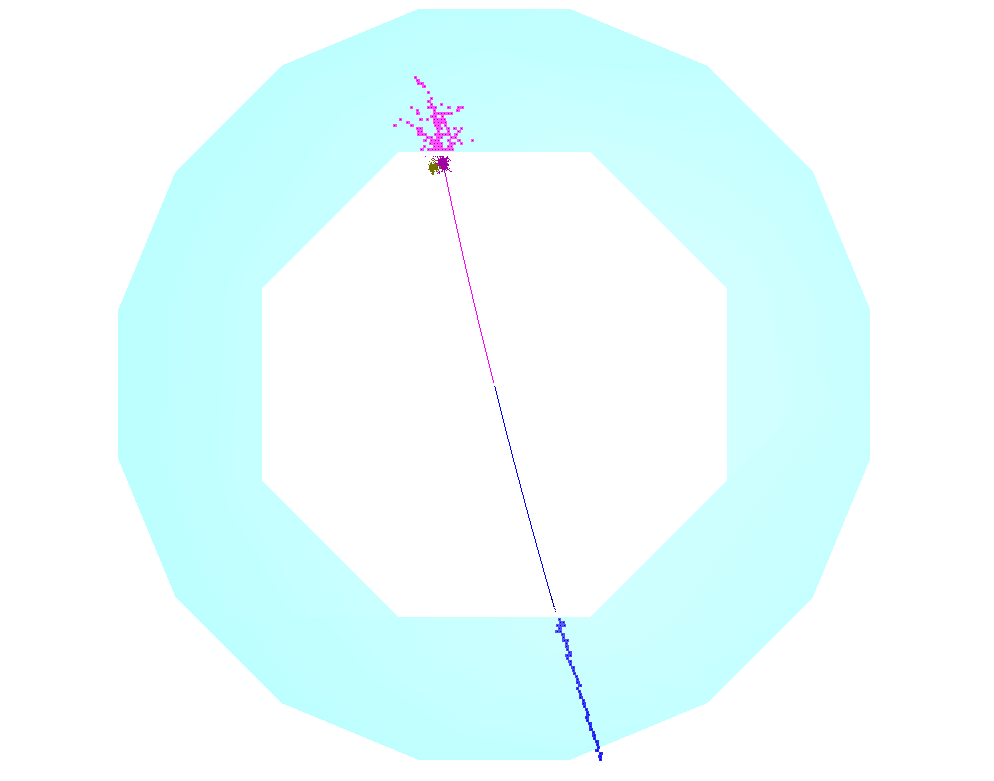
\includegraphics[width=0.5\textwidth]{images/tautauMod}}%

\caption{An event display of a simulated $\Pem\Pep\to \Ptauon\APtauon$ event. The blue region is the cross section of the Electromagnetic Calorimeter barrel region. The top $\Ptau$ decays into a charged $\Ppi$, two photons and neutrinos. The bottom $\Ptau$ decays into a muon and neutrinos.}
\label{fig:Tautau}
\end{figure}

Photon reconstruction is an important part of particle reconstruction. For many physics processes involving particles decaying into photons, such as $\Ptau$ lepton and $\Ppizero$, a good photon reconstruction, which provides a good single photon completeness and purity, as well as a good photon separation resolution, is crucial for reconstructing these particles.

\end{comment}

%\section{Electromagnetic shower}

\section{Overview of photon reconstruction in \pandora}

\pandora provides a framework for particle reconstruction \cite{Marshall:2015rfa}, as described in \Section{sec:pandoraPandoraPFA}. In the linear collider user case, it has a vast library of algorithms developed over years by many people. Each algorithm addresses one topological issue in the particle reconstruction. The essential part of the \pandora is track-cluster association  to find the best track-cluster pair, and re-clustering to find the best cluster consistent with the track. Other algorithms that identifying trackless clusters, such as muon clusters or photon clusters, would provide a cleaner environment for the track-cluster association, hence improving the jet energy resolution.

Photon identification in \pandora has two main mechanisms. The basic mechanism performs photon identification at the last step of the reconstruction  (see \Section{sec:pandoraPFOcreation}). The second more sophisticated photon identification is performed at an early stage of the reconstruction  (see \Section{sec:particleID}). This algorithm identifies photon electromagnetic shower cores carefully in the dense jet environment. By removing the photons from the environment, fewer calorimeters hits are left for the charged particle reconstruction. Hence the overall reconstruction improves.

The photon reconstruction algorithm in \pandora version 1 improves jet energy resolution by correctly identifying photon electromagnetic shower cores and leaving a cleaner environment for the track-cluster association. However, the peripheral calorimeter hits to the shower cores may be left as fragments, and reconstructed as separate particles. This lowers the reconstructed photon completeness and makes the number of reconstructed photons a less useful physical quantity. Also, the algorithm in \pandora version 1 leaves rooms for improvement of photon separation resolution.

This section presents a solution to the photon reconstruction issue. The newly introduced \pandora algorithms also reduces photon fragments and improves the photon separation resolution. Some part of the work has been published in a conference proceeding \cite{Xu:2016rcz}.

Firstly the algorithm for photon reconstruction will be described, followed by fragment removal algorithms and photon splitting algorithms. This chapter will end with the performance of these photon related algorithms,  including comparisons with the previous photon algorithms.
%Algorithms related to photon reconstruction, fragmental removal and photon splitting, which are written or introduced by authors, will be discussed below.


%The testing simulated data in this paper are generated either by WHIZARD \cite{whizard} or by the simple HepEvt generator. Events are simulated with GEANT4 \cite{Agostinelli:2002hh} in MOKKA \cite{MoradeFreitas:2002kj}. Jet fragmentation was performed with PYTHIA \cite{Sjostrand:1995iq} and the particle reconstruction was done by PandoraPFA \cite{Marshall:2015rfa} in MARLIN reconstruction framework \cite{Gaede:2006pj}, in ILD\_o1\_v6 detector model. The iLCSoft v17-01-07 was used. Different versions of PandoraPFA were used for the comparison purpose.

\section{Electromagnetic shower}
\label{sec:photonEMshower}
A electromagnetic (EM) shower refers to the pair production and bremsstrahlung when a high energy photon or electron passing though a thick absorber. The interaction generates more low energy photons and electrons, producing a shower-like  structure. Two suitable length scales to describe the EM shower are radiation length and \RM. A radiation length of a material is used to describe the longitudinal shower profile, defined as the mean distance travelled where an electron loses its energy by a factor of $1/e$ via bremsstrahlung. It is also defined as the mean free path  for pair production by a high energy photon\cite{segre1977nuclei}. A \RM is used to describe the transverse shower profile.

\begin{figure}[tbph]
\centering
{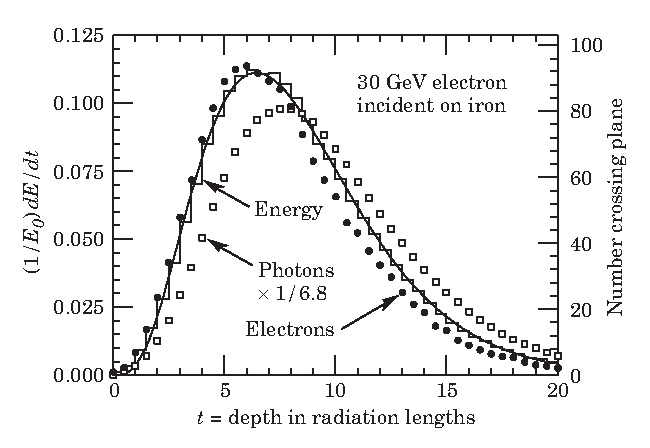
\includegraphics[width=0.45\textwidth]{photon/EMlong}}
\caption[Simulated longitudinal electromagnetic shower profile as a function of depth for electrons and photons.]
{An EGS4 simulation of a 30\,GeV electron-induced electromagnetic shower in iron. The histogram shows fractional energy deposition as a function of radiation lengths, and the curve is a gamma-function fit to the distribution. Circles and squares are the number of electrons and photons respectively with total energy greater than 1.5\,MeV crossing planes with scale on right. Plot is taken from \cite{Agashe:2014kda}.}
\label{fig:photonEMlongProfile}
\end{figure}

\FIGURE{fig:photonEMlongProfile} shows simulated longitudinal electromagnetic shower profile as a function of radiation length for electrons and photons. The mean EM longitudinal shower profile can be described by the following function \cite{Longo:1975wb} :
\begin{equation}
\frac{dE}{dt} = E_0 b \frac{{bt}^{a-1}e^{-bt}}{\Gamma(a)},
\end{equation}
where $t$ is number of radiation lengths. $a$ and $b$ are free parameters. $E_0$ is the shower energy. $b$ varies slightly with material but it is sufficient to use $b = 0.5$. $a$ can be calculated and is:
\begin{equation}
a = 1.25 + 0.5ln\left(\frac{E_0}{E_c}\right),
\end{equation}
where $E_c$ is the critical energy. This parametrisation should only be used to describe an average behaviour of the EM shower, as the fluctuation is important. For the photon identification, a comparison with the parametrisation is used.

The transverse shower profile is a narrow cone widening as the shower develops. 90\% of the energy  is contained in a fiducial cylinder of 1 \RM. Transverse profile is often represented by a sum of two Gaussian function. This allows the two dimensional peak finding to separate EM showers using transverse shower profile.

\section{\PhotonReconstruction algorithm}
\label{sec:photonRecostrcution}

The \PhotonReconstruction algorithm refers to the more sophisticated photon identification at the early stage of the reconstruction. It corresponding to ``Particle ID'' stage \Section{sec:particleID} in the \pandora reconstruction chain.  The main steps of \PhotonReconstruction are: coarsely forming photon clusters, finding photon candidate, photon ID test, and optional fragment removals. The step of finding photon candidate uses   a   two dimensional peak finding algorithm, which requires further explanation in \Section{sec:peakFinding}. The photon ID test involves a multi dimensional likelihood classifier, which is described in \Section{sec:photonLikelihood}. The optional fragment removal algorithm shares a common base case with another photon fragment removal algorithm. Hence they are discussed together in \Section{sec:photonFragRemoval} . A flow diagram of the \PhotonReconstruction algorithm is shown in \Figure{fig:photonPhotonRecoFlow}.

\begin{figure}[tbph]
\centering
{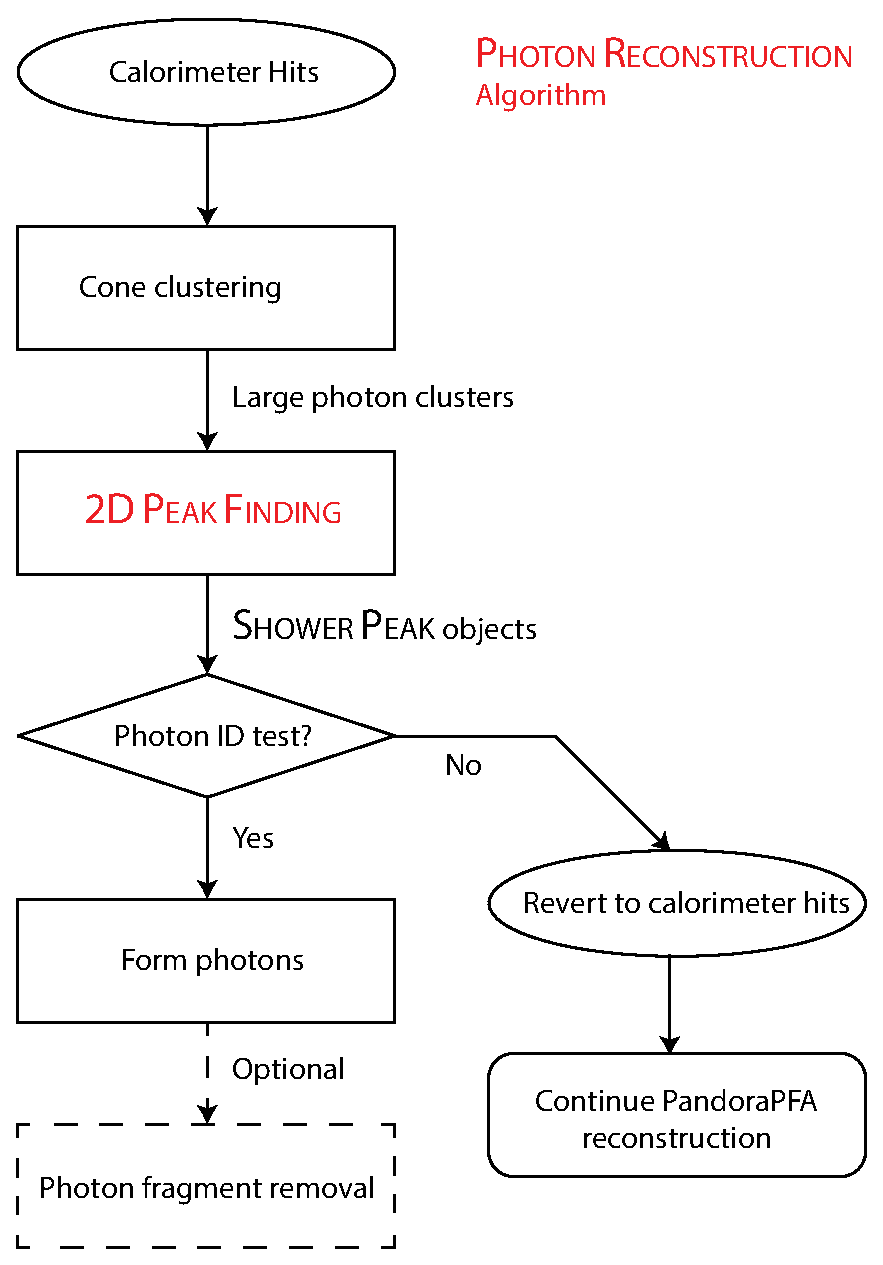
\includegraphics[width=0.45\textwidth]{photon/photonRecoFlow}}
\caption[A flow diagram of the \PhotonReconstruction algorithm.]
{A flow diagram of the \PhotonReconstruction algorithm.}
\label{fig:photonPhotonRecoFlow}
\end{figure}


\subsection{Form photon clusters}

The input of the \PhotonReconstruction algorithm is a collection of calorimeter hits. Muon clusters have been removed prior to this step.  This step finds large potential photon clusters in the \ECAL, which may contain multiple photons. For simplicity, the algorithm opts to reuse  the cone clustering algorithm (see \Section{sec:pandoraConeCluster}) provided inside \pandora to find large clusters. Since the target for reconstruction is neutral electromagnetic shower in the \ECAL, the cone cluster algorithm is set to use high energy calorimeter hits as initial seeds.  The parameters for the cone clustering are generous, forming large clusters for further process.

\subsection{Find photon candidates}
\label{sec:photonCandiate}

The next stage is to refine the large photon clusters into smaller photon candidate. Each photon candidate should contain calorimeter hits from one particle only. The aim for  this step is to split a three dimensional cluster into several smaller cluster. The three dimensional splitting problem is hard. Therefore, a translation is needed to map the three dimensional problem to a more manageable two dimensional problem. The translation relies on the on the characteristic electromagnetic (EM) showers in the transverse distribution. When an energetic photon or electron hits the absorber layers of the \ECAL, it initiates an electromagnetic shower, where electron pair production and bremsstrahlung produce more low-energy photons and electrons. The transverse distribution is characterised by a narrow cone, widening while the shower develops. Therefore, along the direction of the photon shower, an  EM shower appears as a dense core with peripheral hits. If the energy deposition is projected on to a plane, the EM shower core would appear as a peak. By identifying a peak in the two dimensional plane, the EM shower core is identified.  Hence with the projection translation, three dimensional cluster splitting problem is mapped to a two dimensional peak finding problem. \Figure{fig:photonPeakFinding} shows an example of a large photon cluster projected on to a two dimensional plane.

%the energy deposition projection of two photons candidates. U and V axis are two arbitrary orthogonal axis in the transverse plane perpendicular to the direction of photons. Z axis shows the sum of the calorimeter hit energy in GeV. The bin size corresponds to the square \ECAL cell size.


%To reduce the problem of splitting a three dimensional clusters (a collection of hits) into a manageable two dimensional problem.

%The large photon clusters are split into smaller photon candidates, using two-dimensional shower profiles. The candidates close to a track projection are deemed as non-photons. Identifying photon candidates within a large photon cluster relies on the characteristic electromagnetic showers, in particular the transverse distribution. A energetic photon or electron hits the absorber layers of the \ECAL, it initiates an electromagnetic shower, where electron pair production and bremsstrahlung produce more low-energy photons and electrons. The transverse distribution is characterised by a narrow cone, widening while the shower develops.

%To view the transverse shower distribution, a two-dimensional energy deposition projection is constructed in the plane perpendicular to the direction of the cluster. \Figure{fig:photonPeakFinding} shows the energy deposition projection of two photons candidates. U and V axis are two arbitrary orthogonal axis in the transverse plane perpendicular to the direction of photons. Z axis shows the sum of the calorimeter hit energy in GeV. The bin size corresponds to the square \ECAL cell size.

\begin{figure}[tbph]
\centering
{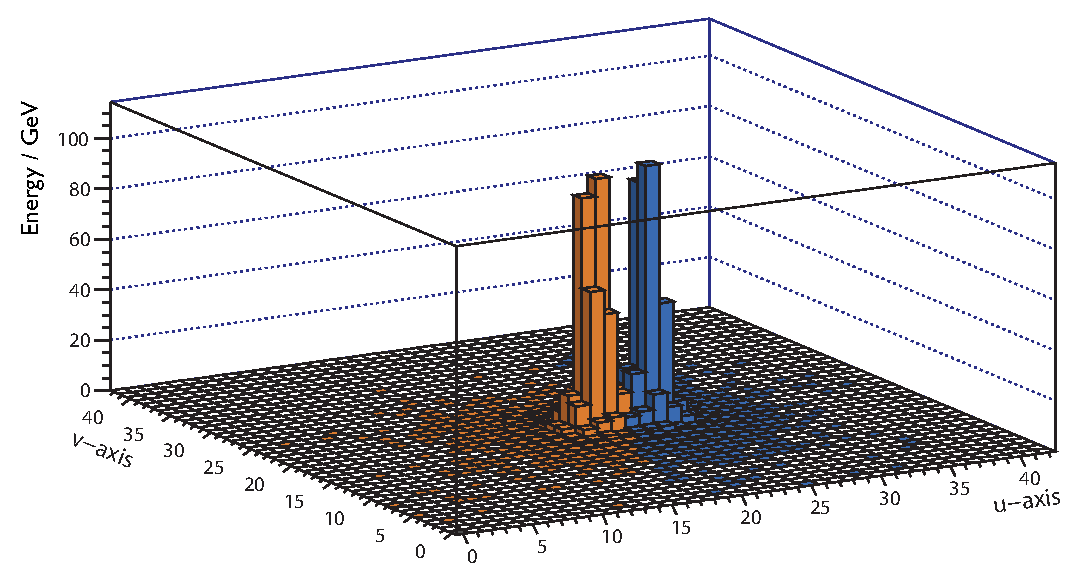
\includegraphics[width=0.5\textwidth]{photon/peakFindingMod}}
\caption[Example of a projection of a large photon clusters containing two photons.]
{Two 500\,GeV photons (yellow and blue), just resolved in the transverse plane perpendicular to the direction of the flight, of their energy deposition in the electromagnetic calorimeter. U and V are orthogonal axes. Z axis is the sum of the calorimeter hit energy in each particular bin in GeV.}
\label{fig:photonPeakFinding}
\end{figure}

By using the two-dimensional energy deposition projection, separating photons translates to separating peaks in the projection. Therefore a high performance two dimensional peak finding algorithm is the key to identify multiple photons. Due its complexity, the peak finding algorithm is discussed separately in \Section{sec:peakFinding}. The output of the two dimensional peak finding is a collection of \ShowerPeak objects. Each \ShowerPeak object corresponds to a photon candidate and contains associated calorimeter hits.

\subsection{Photon ID test}
\label{sec:photonIDtest}

\ShowerPeak objects are tested for photon tagging.  A set of discriminating variables that exploit features electromagnetic showers are calculated. A multidimensional likelihood classifier is implemented, which would be trained before applying. The response from the classifier determines if a \ShowerPeak object is a photon. If it is a photon, it would be tagged and separated out from the event. If it is not a photon, the calorimeter hits of the \ShowerPeak object will be passed on to the next stage of the reconstruction. Because the classifier is complicated, it is discussed in separate \Section{sec:photonLikelihood}.

\subsection{Photon Fragment removal}
\label{sec:photonRecoFragRemoval}

The optional photon fragment removal aims to merge small photon fragment to identified photons. Since this step shares the same logic as the fragment removal algorithm in \Section{sec:photonFragRemoval}, the description of the fragment removal algorithm is delayed to \Section{sec:photonFragRemoval}.

%only differing in the cut-off values for merging metrics, this step be discussed in \Section{}.

This step marks the end of the photon reconstruction algorithm. The output are a collection of reconstructed photons, separated from non-photon calorimeter hits. \FIGURE{fig:photonPhotonRecoFlow}  summarise key steps in the \PhotonReconstruction algorithm.
%The candidate passed the test will be kept in a separate container for photons only

\section{Two dimensional peak finding algorithm for photon candidate}
\label{sec:peakFinding}

As discussed in \Section{sec:photonCandiate}, separating photon candidates from a cluster is same as identifying peaks in a two dimensional histogram. An example of two photons is shown in the \Figure{fig:photonPeakFinding}. The \peakFinding algorithm aims to correctly identify peak positions in a two dimensional histogram and associate other bins. A flow chart for the algorithm is shown in \Figure{fig:photonPeakFindingFlowNeutral}.

The base algorithm treats all clusters as potential photon clusters, hence the neutral cluster variant. Since charged hadrons would deposit tracks in the tracking system, extra care is taken when a cluster is close to the projection of the track in the front of the \ECAL. The neutral cluster variant is described first, followed by the modification for charged cluster variant.

\begin{figure}[tbph]
\centering
{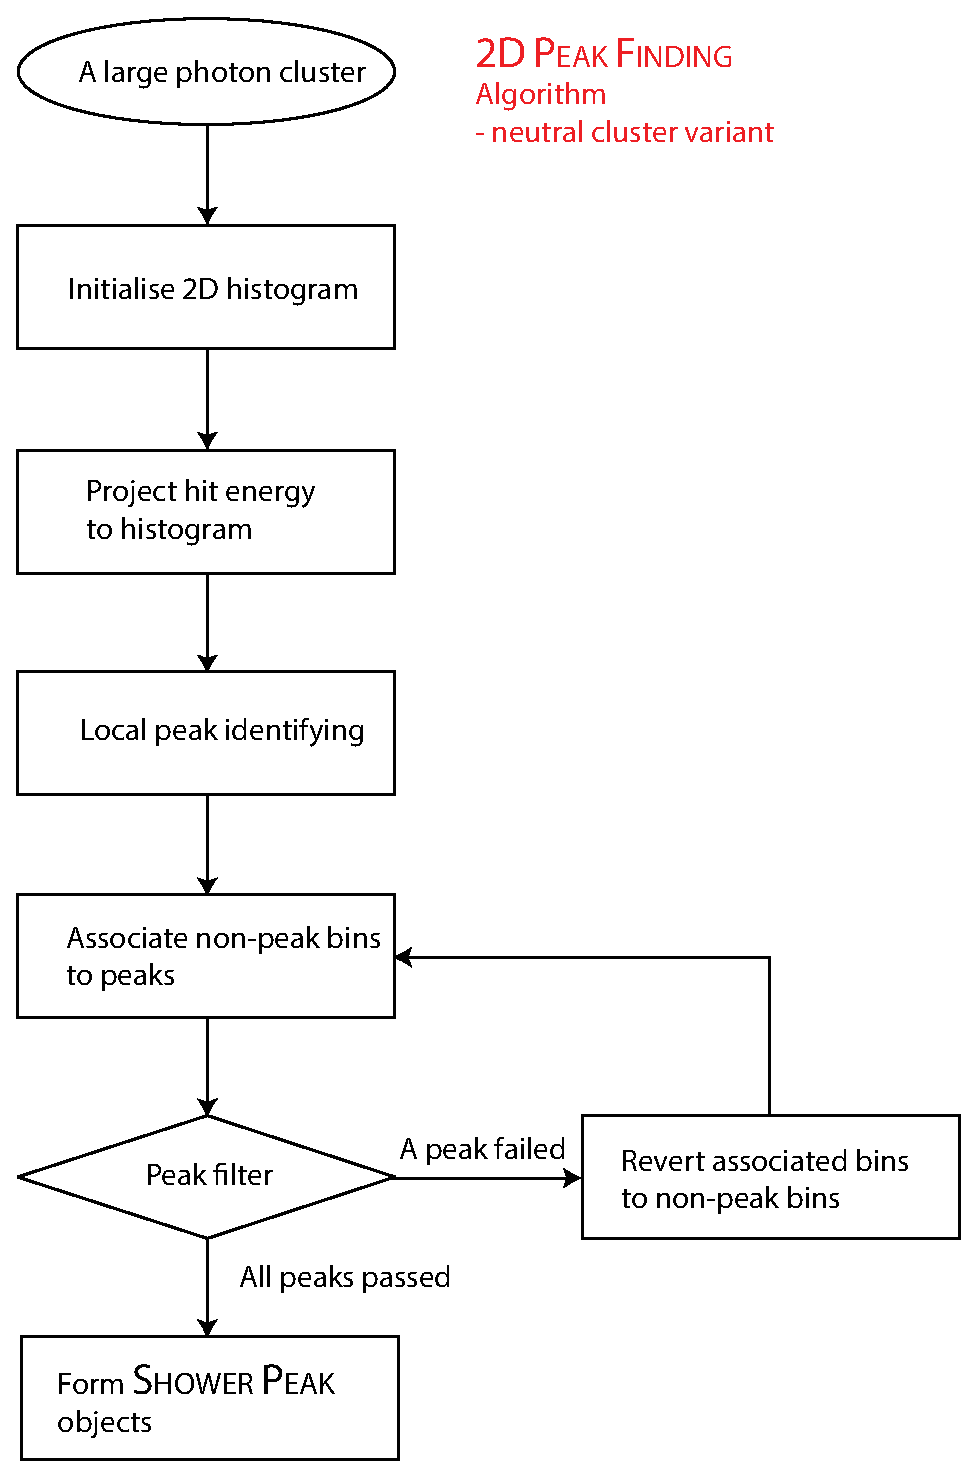
\includegraphics[width=0.5\textwidth]{photon/2DpeakFinding}}
\caption[Flow chart for \peakFinding algorithm neutral cluster variant.]
{Flow chart for \peakFinding algorithm neutral cluster variant.}
\label{fig:photonPeakFindingFlowNeutral}
\end{figure}

\subsection{Initialise 2D histogram}

A two dimensional histogram is initialised. For the best resolving power between photons, the projection direction is chosen to be cluster's direction. Therefore, two axes for the 2D histogram are chosen such that axes and the direction form a orthogonal bases in three dimensional space. The axes are labelled as  U and V axis in \Figure{fig:photonPeakFinding}.



\subsection{Project hit energy to histogram}

This step projects calorimeter hits positions onto the 2D histogram defined in previous step. For a finite sized 2D histogram, the projection is chosen such that the cluster centroid position is at the centre of the histogram. The bin size corresponds to one \ECAL square cell length. The relative distance between the calorimeter hit position is switched into a two dimensional coordinates, and subsequently projected onto the histogram. The coordinate of a hit can be obtained by:
\begin{equation}
\vec{s_{i}} = \frac{\vec{a_{i}} -  \vec{\angles{a}}}{d_{cell}},
\end{equation}
where $\vec{a}$ is the position of the hit $i$.  $\vec{\angles{a}}$ is the centroid position of cluster $a$. $d_{cell}$ is the  \ECAL square cell length. $\vec{s_{i}}$ is pojected to U and V axes via the sclar product.

The projected position on the 2D histogram is binned at integer values. The bin height is the sum of the calorimeter hits energy in that particular bin. The issue with a finite histogram size is discussed in \Section{sec:photonPeakFindingInclusive}.

\subsection{Local peak identifying}

This step identifies all local peaks in the 2D histogram. For example, in \Figure{fig:photonPeakFinding}, there are clearly two peaks, both colour coded. A local peak is defined as a bin where its height is above all eight neighbouring bin. The 2D histogram is linearly scanned. Hence the processing time is $O\left(N^2\right)$, where $N$ is number of bins in one axis.

\subsection{Associate non-peak bins to peaks}

Having tagged all local peaks, this step associates non-peak bins to peaks. A high energy EM shower has a wider shower width. And EM shower is typically narrow transversely. These determine the choice of the metric for associating bins. After all local peak bins are found, non-peak bins are associated to a peak bin, by choosing the peak bin that minimise the metric
\begin{equation}
\frac{d}{\sqrt{E_{peak}}}
\end{equation}
where $d$ is the Euclidean distance between a non-peak bin and a peak bin on the histogram, and $E_{peak}$ is the height of the peak bin. Alternative metrics provided in the algorithm include $d$, $\frac{d}{{E_{peak}}}$, and $\frac{d}{{E_{peak}^2}}$. The default metric is chosen due to a good balance between distance and energy of the peak.

\subsection{Peak filtering}

The performance of the two dimensional peaking finding algorithm is improved by clever programming and physics arguments. For a given two dimensional histogram, such as the one in \Figure{fig:photonPeakFinding}, major peaks most likely correspond to physical photons, while the minor peaks more likely come from fluctuations in energy deposition. To select major peaks, every time after non-peak bins are associated with peak bins, minor peaks with fewer than three bins associated (including the peak bin) are discarded. These bins are re-associated with other peak bins. This iterative process stops when all peak bins have at least three bins associated.  The algorithm also allows bins with height below a critical value to not participate in the peak finding. The default value is set such that only empty bins are not used.

The output are \ShowerPeak objects. Each contains one peak bin and its associated bins, along with the calorimeter hits in bins and derived quantities of the peak.

\subsection{Candidate close to track projection}

If a cluster or a photon candidate is close to the projection of the track in the front of the \ECAL, it is likely that the cluster or the candidate is a charged hadron. Misidentifying a charged hadron as a photon leads to significant degradation in reconstruction performance. However, if a photon next to a charged hadron is carefully reconstructed, the overall reconstruction is improved. Hence this step aims to carefully identifies photon candidate next to charged hadrons, by using track information and features of the electromagnetic shower. Photon induced electromagnetic shower in the \ECAL typically start in the first few layers. As the shower develops, the direction of the shower core does not change much.

\begin{figure}[tbph]
\centering
{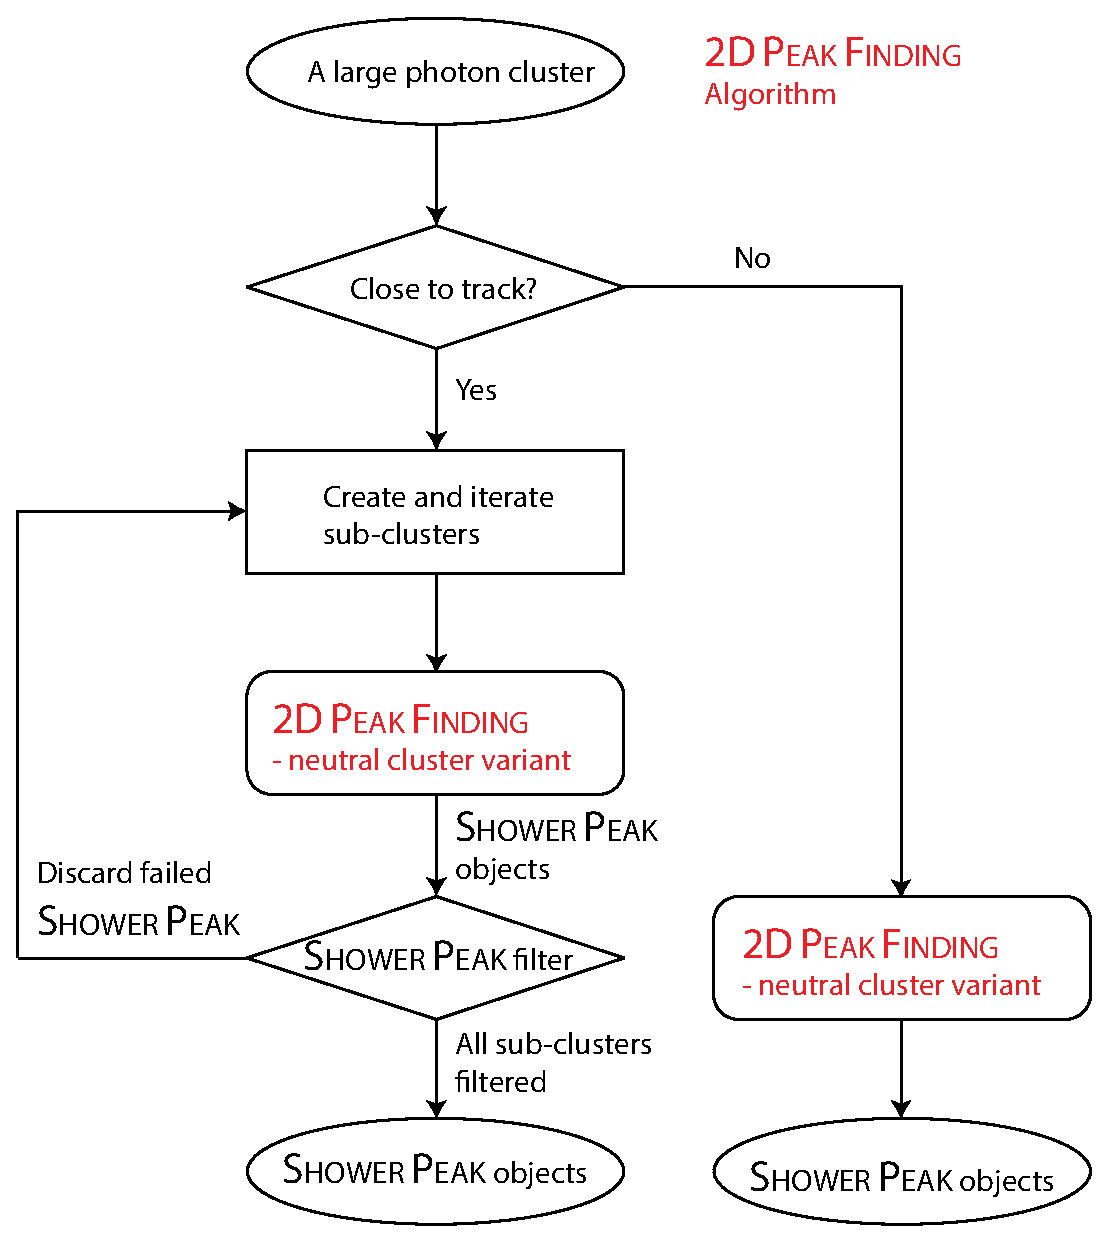
\includegraphics[width=0.5\textwidth]{photon/2DpeakFindingTrack}}
\caption[Flow chart for \peakFinding algorithm.]
{Flow chart for \peakFinding algorithm.}
\label{fig:photonPeakFindingFlow}
\end{figure}

\FIGURE{fig:photonPeakFindingFlow} shows the flow chart for the full \peakFinding algorithm, including the treatment with clusters close to tracks. If a cluster is less than 3\,mm from the closest track projection, it is treated as a potentially charged cluster. The \ECAL is sliced longitudinally to help identify photon candidates. For example, the default three slices will result in three \ECAL fiducial spaces, each contains space from the front of the \ECAL to a third, two thirds and the back of the \ECAL, respectively. The peaking finding algorithm is repeated for the sub-cluster contained in each fiducial space. The peak is only preserved as a photon candidate if the peak exists in every fiducial space, and if its position is shifted by no more than one neighbouring bin between fiducial spaces. Furthermore, if a peak bin is within the eight neighbouring bins of the track projection onto the two dimensional plane, the peak and its associated bins are flagged as charged particles, non-photons.

\subsection{Inclusive mode}
\label{sec:photonPeakFindingInclusive}

The two dimensional histogram is iterated during the algorithm. The time complexity is $O(n^2)$ for a $n \times n$ histogram (Default $n = 41$). Therefore, for the purpose of speed, it is undesirable to have a very large histogram. However, since the histogram has a finite size, only energy deposition projected on the histogram would be considered for peak finding. When \ShowerPeak objects are constructed, calorimeter hits outside the histogram would be lost. This behaviour is suitable for photon reconstruction (\Section{sec:photonCandiate}) and test for photon fragment removal (\Section{sec:photonFragRemoval}). However, for photon splitting (\Section{sec:photonSplitting}), there should be no calorimeter hits loss from splitting a photon. Hence inclusive mode of the peak finding algorithm is developed, and it allows energy deposition projected outside the histogram to be associated with identified peaks.


\section{Likelihood classifier for photon ID}
\label{sec:photonLikelihood}

\SECTION{sec:photonIDtest} outlines the photon ID test in the photon reconstruction algorithm. This section describes the multidimensional likelihood classifier in details, including discriminating variables. For each photon candidate, a set of kinematic variables are calculated.

\subsection{Overview of Projective Likelihood}
\label{sec:photonPDE}
Projective likelihood model (PDE) is used in \pandora for the photon ID due to its simplicity and low requirement on computing resources.

PDE implemented calculates the probability density for each discriminative variable, for signal and background. The overall signal and background likelihood are defined as products of the individual probability density. The likelihood ratio, $R$, is then defined as the signal likelihood over signal plus background likelihood.

To use the likelihood ratio, one way is to fit an underlying function to the probability density, which is implemented the \TMVA software package. The other way is to use binned likelihood ratio, $R$, as the output, due to the simplicity. This is implemented in the \pandora. Similarly to classifier like the rectangular cut method, PDE works better with decorrelated, gaussian like variables. The \pandora implementation does not decorrelate nor transform the variables, to keep implementation fast.

\subsection{Projective Likelihood in \pandora}

Kinematic variables exploit the differences between a characteristic electromagnetic shower and a hadronic shower, and the fact that a photon is more likely to be isolated from other showers and charged tracks. A full list of variables can be found in \Table{tab:photonPhotonIDvar}.

\begin{table}[htbp] \centering \smallskip
\begin{tabular}{l r }
\hline
Categories&  Variables\\
\hline
Longitudinal shower profile & $\delta{l}$,$t_0$ \\
Transverse shower profile & $\langle{w}\rangle$,$\delta{\langle{w_{UV}}\rangle}$, $\delta E_{cluster}$ \\
Distance to track &  $d$ \\
\hline
\hline
\end{tabular}
\caption
{List of variables for the photon likelihood base ID test.}
\label{tab:photonPhotonIDvar}
\end{table}

Two variables use the longitudinal shower distribution. $t_0$ is the start layer from the longitudinal shower profile (see \Section{sec:photonEMshower}). $\delta{l}$ is fractional difference from the expected shower profile \cite{Thomson:2009rp}:
\begin{equation}
\delta l = \frac{1}{E_0}\sum_{i}^{}\absOf{\Delta E_{obs}^i - \Delta E_{EM}^i }.
\end{equation}
$\delta l$ is minimised as a function of the $t_0$.

Three variables use the transverse shower information. $\langle{w}\rangle$ is the energy weighted r.m.s. bin distance to the peak bin. This is a measure of the peak size. $\delta{\langle{w_{UV}}\rangle}$ is the smallest ratio of the two r.m.s. distances in each axis direction, a measure of the circularity of the transverse shower. Last variable, $\delta E_{cluster}$, is the  ratio between the photon candidate energy to the photon cluster energy. This is a measure of the dominance of a photon in a large cluster. Last variable is the distance between the photon candidate and the closest track projection. It is less likely to be a photon if it is close to a track.

The distributions of these variables are normalised to probability distribution, stored in binned histograms. The classifier is improved by realising the kinematic variable distributions varies with photon energies. Thus these distributions are divided by bins of photon candidate energy. The default energy bins edges are 0.2, 0.5, 1, 1.5, 2.5, 5, 10, 20\,GeV, which covers a good range of photon energies. Candidate with energy below 0.2\,GeV would not be examined in this step, as it is very unlikely to be a photon. The classifier training typically uses simulated 250\,GeV jet events. High energy jets allow the training for high energy photon candidates

After training, for a given candidate, the likelihood classifier output is given by
\begin{equation}
pid = \frac{N\prod_{i}{P_i}}{N\prod_{i}{P_i} + N'\prod_{i}{P'_i}}
\end{equation}
where $P_i$ and $P'_i$ are the probability of $i^{th}$ kinematic variable of photon and non-photon candidates. $N$ and $N'$ are the number photon and non-photon candidates.

During classification, a candidate passes the photon id test if
\begin{equation}
\begin{cases}
  pid > 0.6, & \text{if}\ 0.2 < E < 0.5\,GeV\\
  pid > 0.4, & \text{if}\ E \geqslant 0.5\,GeV
\end{cases}
\end{equation}
where $E$ is the candidate energy. Two values of the $pid$ cuts reflect the confidence of the id test with different candidate energy. The test is more cautious with low energy candidate.


\section{Photon fragment removal algorithm in the \ECAL}
\label{sec:photonFragRemoval}
During the reconstruction, it is possible that a core of the photon electromagnetic shower is identified as a photon (the main photon). The outer part of the shower is reconstructed as a separate particle, and wrongly identified as a photon or a neural hadron (the photon/neutral fragment). \Figure{fig:photonEvtDspPhotonFrag} shows a typical creation of such a photon fragment. The fragment does not have the electromagnetic shower structure, and typically it is has much lower energy than the main photon. If a photon-fragment pair is merged, the pair should be consistent with a one-particle profile. These characteristics are used to merge fragments to main photons.

\begin{figure}[tbph]
\centering

  \begin{subfigure}[b]{0.3\textwidth}
    
\includegraphics[width=\textwidth]{photon/allPhoton}
    \caption{}
    \label{fig:photonEvtDspPhotonFragAll}
  \end{subfigure}
  \begin{subfigure}[b]{0.3\textwidth}
    
\includegraphics[width=\textwidth]{photon/big}
    \caption{}
    \label{fig:photonEvtDspPhotonFragBig}
  \end{subfigure}
  \begin{subfigure}[b]{0.3\textwidth}
    
\includegraphics[width=\textwidth]{photon/small}
    \caption{}
    \label{fig:photonEvtDspPhotonFragSmall}
  \end{subfigure}

\caption
{An event display of a typical 10\,GeV photon (\Figure{fig:photonEvtDspPhotonFragAll}), reconstructed into a main photon (\Figure{fig:photonEvtDspPhotonFragBig}) and a photon fragment (\Figure{fig:photonEvtDspPhotonFragSmall}). }
\label{fig:photonEvtDspPhotonFrag}
\end{figure}


Photon fragment removal algorithms can exist in multiple step in the reconstruction: at the end of the \PhotonReconstruction algorithm (see \SECTION{sec:photonRecoFragRemoval}), or at the end of the \pandora reconstruction. Since these algorithms share the same base class, they will be discussed together. The latter algorithm will be discussed. The former algorithm differs mostly in the default cut-off values for merging metrics.


Spatially close photon and a potential fragment form a pair of particles (photon-fragment pair). Kinematic and topological properties of a photon-fragment pair are examined. The pair is merged when the properties pass a set of cuts, developed by comparing true photon-fragment pairs and non photon-fragment pair. This merging test is iterated over all possible  photon-fragment pairs. If multiple photon-fragment pairs pass the merging test, the pair with closest distance metric, $d$, will be merged, shown \Figure{fig:photonDistanceMetric}.

\begin{figure}[tbph]
\centering
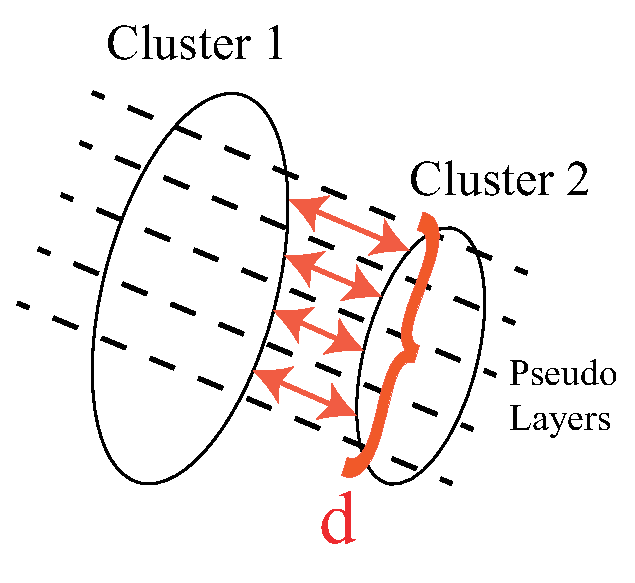
\includegraphics[width=0.45\textwidth]{photon/dLayer}
\caption{Illustration of distance metric, $d$.}
\label{fig:photonDistanceMetric}
\end{figure}


The photon-fragment pairs is classified into photon-photon-fragment pairs and photon-neutral-hadron-fragment pairs, because they have different kinematic and topological distributions. The pairs are further classified into low energy and high energy pair, depending on whether the fragment energy ($E_p$) above 1\,GeV. The cuts for merging pairs, are classified which will be explained later, are listed in \Table{tab:photonFragRemovalCuts}.

\begin{table}[htbp]
\centering

\smallskip

\begin{tabular}{l  r  r }
\hline
Low $E_f$ &  Photon-photon & Photon-neutral-hadron \\
\hline
\multicolumn{1}{L{0.3\textwidth}}{transverse shower comparison} & \multicolumn{1}{R{0.3\textwidth}}{$d < 30 $, $\frac{E_{p1}}{E_m + E_f} > 0.9 $, $\frac{E_{p2}}{E_f} < 0.5 $, $E_{p1} > E_m$}  & \multicolumn{1}{R{0.3\textwidth}}{-} \\
\multicolumn{1}{L{0.3\textwidth}}{close proximity} & \multicolumn{1}{R{0.3\textwidth}}{-}  & \multicolumn{1}{R{0.3\textwidth}}{$d < 20 $, $d_c < 40 $} \\
\multicolumn{1}{L{0.3\textwidth}}{low energy fragment} & \multicolumn{1}{R{0.3\textwidth}}{$d < 20 $, $E_p < 0.4 $}  & \multicolumn{1}{R{0.3\textwidth}}{-} \\
\multicolumn{1}{L{0.3\textwidth}}{small fragment 1} & \multicolumn{1}{R{0.3\textwidth}}{$d < 30 $, $N_{calo} < 40 $, $d_c < 50 $}  & \multicolumn{1}{R{0.3\textwidth}}{$d < 50 $, $N_{calo} < 10 $, $d_h < 50$} \\
\multicolumn{1}{L{0.3\textwidth}}{small fragment 2} & \multicolumn{1}{R{0.3\textwidth}}{$d < 50 $, $N_{calo} < 20 $}  & \multicolumn{1}{R{0.3\textwidth}}{-} \\
\multicolumn{1}{L{0.3\textwidth}}{small fragment forward region} & \multicolumn{1}{R{0.3\textwidth}}{$N_{calo} < 40$, $d_c < 60$, $E_f < 0.6$, $\absCosTheta > 0.7$}  & \multicolumn{1}{R{0.3\textwidth}}{-} \\
\multicolumn{1}{L{0.3\textwidth}}{relative low energy fragment} & \multicolumn{1}{R{0.3\textwidth}}{$d < 40$, $d_h < 20$, $\frac{E_{f}}{E_m} < 0.01$}  & \multicolumn{1}{R{0.3\textwidth}}{$d < 40$, $d_h < 15$, $\frac{E_{f}}{E_m} < 0.01$} \\
\hline
High $E_f$ &  Photon-photon & Photon-neutral-hadron \\
\hline
\multicolumn{1}{L{0.3\textwidth}}{transverse shower comparison} & \multicolumn{1}{R{0.3\textwidth}}{$\frac{E_{p1}}{E_m + E_f} > 0.9 $, $E_{p2} = 0$ or ($\frac{E_{p2}}{E_f} < 0.5 $, $E_{p1} > E_m$)}  & \multicolumn{1}{R{0.3\textwidth}}{$\frac{E_{p1}}{E_m + E_f} > 0.9 $, $E_{p2} = 0$ or ($\frac{E_{p2}}{E_f} < 0.5 $, $E_{p1} > E_m$)} \\
\multicolumn{1}{L{0.3\textwidth}}{relative low energy fragment 1} & \multicolumn{1}{R{0.3\textwidth}}{$d < 40$, $d_h < 20$, $\frac{E_f}{E_m} < 0.02$} & \multicolumn{1}{R{0.3\textwidth}}{$d < 40$, $d_h < 20$, $\frac{E_f}{E_m} < 0.02$} \\
\multicolumn{1}{L{0.3\textwidth}}{relative low energy fragment 2} & \multicolumn{1}{R{0.3\textwidth}}{-}  & \multicolumn{1}{R{0.3\textwidth}}{$d < 40$, $d_h < 20$, $\frac{E_f}{E_m} < 0.1$, $E_f > 10$} \\
\multicolumn{1}{L{0.3\textwidth}}{relative low energy fragment 3} & \multicolumn{1}{R{0.3\textwidth}}{-}  & \multicolumn{1}{R{0.3\textwidth}}{$d < 20$, $d_h < 20$, $\frac{E_f}{E_m} < 0.2$, $E_f > 10$} \\
\hline

\hline
\end{tabular}

\caption[The cuts for photon fragment removal algorithm in the \ECAL.]%
{The cuts for merging photon-photon-fragment pairs and photon-neutral-hadron-fragment pairs for both low energy and high energy fragments. $d$, $d_c$ and $d_h$ are the mean energy weighted intra-layer distance of the pair, the distance between centroids, the minimum distance between calorimeter hits of the pair. $E_m$ and $E_f$ are the main photon energy and the fragment energy. $E_{p1}$ and $E_{p2}$ are the two largest peaks, found by peak finding algorithm, ordered by descending energy. $N_{calo}$ is the number of the calorimeter hits in the fragment. $\absCosTheta$ is the absolute cosine of the polar angle, where beam direction is the z-axis.}
\label{tab:photonFragRemovalCuts}
\end{table}

\TABLE{tab:photonFragRemovalCuts} lists cuts for merging photon-photon-fragment pairs and photon-neutral-hadron-fragment pairs for both low energy and high energy fragments. $d$, $d_c$ and $d_h$ are mean energy weighted intra-layer distance within the pair, distance between two centroids, and minimum distance between calorimeter hits of each \PFO in the pair, respectively.  Three distance measurements have subtle difference. $d_c$ gives the distance between centroids of each \PFO in the pair, which is a quick but crude measurement. $d_h$ is the minimum distance between calorimeter hits of each \PFO in the pair. For a true photon-fragment, $d_h$ should be close to zero as the pair should be spatially close. $d$ is the mean energy weighted intra-layer distance between  each \PFO in the pair (see \Figure{fig:photonDistanceMetric}):
\begin{equation}
d = \frac{\sum_{i}^{layers}d_{l,i}\ E_{f,i}}{\sum_{i}^{layers}E_{f,i}}
\end{equation}
where $i$ indicates $i^{th}$ pseudo-layer of the \ECAL. $d_{l,i}$ is the minimum distance between calorimeter hits of the pair in the $i^{th}$ pseudo-layer. $E_{f,i}$ is the energy of the fragment in the the $i^{th}$ pseudo-layer. $d$ is a better measurement of the closeness of the pair. Similar to $d_h$, $d$ will be very small for a true photon-fragment pair.

The close proximity cuts require the distance between pairs to be small.

$E_m$ and $E_f$ are the main photon energy and the fragment energy. $E_{p1}$ and $E_{p2}$ are the two largest peaks and associated calorimeter hits, found by the two dimensional peak finding algorithm (\Section{sec:peakFinding}), ordered by descending energy, using the pair as input. $N_{calo}$ is the number of the \ECAL hits in the fragment. $\absCosTheta$ is the absolute cosine of the polar angle of the main photon, where beam direction is the z-axis.

One logic for merging is when the fragment is small with low energy and is close to the main photon. Hence $E_f$  and $N_{calo}$ are required to be small. Alternatively the fragment should be relatively low energy, demanding a small ratio of $E_f$ to $E_m$.

The other logic is when the pair looks like one photon in two-dimensional energy deposition projection (see \Section{sec:photonCandiate} and \Figure{fig:photonPeakFinding}). The transverse shower comparison requires $\frac{E_{p1}}{E_m + E_f} > 0.9 $, most energy contains in the first \ShowerPeak obkect.

Comparing low $E_f$ and high $E_f$ cut, the cuts are similar. High $E_f$ cuts are more relaxed on the energy comparison for small fragment test. 

Comparing photon-photon-fragment pair and photon-neutral-hadron-pair, cuts for photon-neutral-hadron-pair are more conservative for low $E_f$, but more relaxed for high $E_f$. This reflects that the neutral hadron fragments originated from charged particles are more likely to be low energy, whilst high energy neutral fragments are more likely to be photon fragments. 

Since all possible photon-fragment pairs are compared, this is a costly cooperation with $O(n^2)$ time complexity for $n$ particles. The speed is improved by considering only the pairs with $d<80\text{mm}$. 


\section{High energy photon fragment recovery algorithm}
\label{sec:photonHighEFragRemoval}

\SECTION{sec:photonFragRemoval} descried effective algorithms to removal photon fragments that are peripheral to the main photon, the electromagnetic shower core. An example of such fragment is shown in \Figure{fig:photonEvtDspPhotonFrag}. There is another type of fragment originated from the leakage effect of the \ECAL. When a high energy EM shower is not fully contained in the \ECAL, shower deposits energy in the \HCAL, which often forms a neutral hadron in the \HCAL. Photon reconstruction, as described in \Section{sec:photonRecostrcution}, considers only calorimeter hits in the \ECAL.  An example of a 500\,GeV photon reconstructed into a main photon in the \ECAL (yellow) and a neutral hadron fragment in the \HCAL (blue) is shown in \Figure{fig:photonEvtDspHCalFrag}. For the \ILD detector, this \ECAL leakage effect appears when the photon energy is above 50\,GeV.


\begin{figure}[tbph]
\centering
{
\includegraphics[width=0.5\textwidth]{photon/hcalfrag}}%
\caption{An event display of a typical 500\,GeV photon, reconstructed into a main photon in the \ECAL (yellow) and a neutral hadron fragment in the \HCAL (blue).}
\label{fig:photonEvtDspHCalFrag}
\end{figure}

With \Figure{fig:photonEvtDspHCalFrag} as an example, high energy fragments in the \HCAL is spatially close to the main photon. A fitted cone from the main photon covers most of the fragment if extended to the \HCAL. These features allow a set of cuts developed to merge high energy fragments, listed in \Table{tab:photonHighEnergyFragCuts}

This algorithm would collect the photons and neutral hadrons in the \HCAL as inputs. It occurs after the first pass of topological association in the reconstruction, which connects tracks to clusters in the \ECAL and the \HCAL. The algorithm would iterate over all pairs of reconstructed photons and neutral hadrons in the \HCAL. For each pair, a set of variables are calculated and compared to a set of cuts (\Table{tab:photonHighEnergyFragCuts}). Photon-fragment pairs passing the cuts will be merged.

\begin{table}[htbp]
\centering

\smallskip

\begin{tabular}{l r }
\hline
High energy fragment recovery&  Cuts\\
\hline
\multicolumn{1}{L{0.3\textwidth}}{distance comparison} & \multicolumn{1}{R{0.3\textwidth}}{$d^l_c \leqslant 173\ \text{mm}$, $d^l_{cone} \leqslant 100\ \text{mm}$, $d_{cone} \leqslant 100\ \text{mm}$} \\
\multicolumn{1}{L{0.3\textwidth}}{shower width comparison} & \multicolumn{1}{R{0.3\textwidth}}{$  0.3 \leqslant \frac{w^l_f}{w^l_m} \leqslant 5$} \\
\multicolumn{1}{L{0.3\textwidth}}{projection comparison} & \multicolumn{1}{R{0.3\textwidth}}{$ r_f \leqslant 45\ \text{mm}$} \\
\multicolumn{1}{L{0.3\textwidth}}{energy comparison} & \multicolumn{1}{R{0.3\textwidth}}{$ \frac{E_f}{E_m} \leqslant 0.1$} \\
\multicolumn{1}{L{0.3\textwidth}}{cone comparison} & \multicolumn{1}{R{0.3\textwidth}}{$ \%{N_{calo,cone}} \geqslant 0.5$} \\
\hline

\hline
\end{tabular}

\caption[Cuts for merging high energy photon fragment in the \HCAL.]%
{The cuts for merging high energy photon fragment in the \HCAL to the main photon in the \ECAL. $d^l_c$ is the distance between centroids of the last outer layer of the main photon and the first inner layer of the fragment. $d^l_{cone}$ is the distance between fitted cones using the last outer layer of the main photon and the first inner layer of the fragment. $d_{cone}$ is the distance between fitted cones using the main photon and the fragment. $w^l_m$ and $w^l_f$ are the r.m.s. width of the last outer layer of the main photon and the first inner layer of the fragment. $r_f$ is the r.m.s. mean energy weighted distance of a calorimeter hit in the fragment to the direction of the main photon. $E_m$ and $E_f$ are the main photon energy and the fragment energy. $\%{N_{calo,cone}}$ is the fraction of the calorimeter hits in the fragment in the extended fitted cone of the main photon.}
\label{tab:photonHighEnergyFragCuts}
\end{table}

Fragment in the \HCAL should be spatially close to the main photon, measured by three metrics. $d^l_c$ is the distance between centroids of the last outer layer of the main photon and the first inner layer of the fragment. $d^l_{cone}$ is the distance between fitted cones using the last outer layer of the main photon and the first inner layer of the fragment. $d_{cone}$ is the distance between fitted cones using the main photon and the fragment.

The direction of the fragment should be similar to that of the main photon. $r_f$, the r.m.s. mean energy weighted distance of a calorimeter hit in the fragment to the direction of the main photon, has to be small for merging.

Another feature of the fragment and the main photon is that the shower width should be similar. $w^l_m$ and $w^l_f$ are the r.m.s. width of the last outer layer of the main photon and the first inner layer of the fragment. The ratio $\frac{w^l_f}{w^l_m}$ needs to be in the range of 0.3 to 5. The generous upper bound is due to the \HCAL is coarser than the \ECAL.

When a fitted cone from the main photon is extended to the \HCAL, the cone should contain a significant amount of the fragment. $\%{N_{calo,cone}}$, the fraction of the calorimeter hits in the fragment in the extended fitted cone of the main photon, has to be no less than 0.5 for the merging.

The last criteria is the fragment should has low energy relative to the main photon. $E_m$ and $E_f$ are the main photon energy and the fragment energy. The ratio, $\frac{E_f}{E_m}$, has to be less than 0.1 for the merging.

If multiple photon-fragment pairs pass the cuts with the same fragment, the pair with highest $\%{N_{calo,cone}}$ will be merged.


\section{Photon splitting algorithm}
\label{sec:photonSplitting}

Algorithms described above deal with forming photons from calorimeter hits in the \ECAL, merging photon fragments in the \ECAL and the \HCAL. Another aspect in photon reconstruction is splitting accidentally merged photons. During the particle reconstruction, it is possible that photons are accidentally merged if they are spatially close. Hence another algorithm at the end of the particle reconstruction addresses this issue and tries to split merged photons.

Merged photon is typically energetic. The merged photon should be consistent with topologies of a spatially closed photon pair. Extra care should be taken if the photon is close to a charged \PFO. Many \pandora algorithms deal with track clusters association and there is a greater confidence in clusters associated with tracks. These features form logics behind the algorithm.

\begin{table}[htbp]
\centering

\smallskip
\small
\begin{tabular}{l r }
\hline
Photon splitting&  Cuts\\
\hline
\multicolumn{1}{L{0.3\textwidth}}{Cuts} & \multicolumn{1}{R{0.3\textwidth}}{$E > E_{c1}$, $E_{p2} > E_{c2}$, $N_{p} < 5$} \\
\hline
$E_{c1}$ and $E_{c2}$ values &  \\
\hline
\multicolumn{1}{L{0.3\textwidth}}{0 charged \PFO nearby} & \multicolumn{1}{R{0.3\textwidth}}{$E_{c1} = 10$, $E_{c2} = 1$} \\
\multicolumn{1}{L{0.3\textwidth}}{1 charged \PFO nearby} & \multicolumn{1}{R{0.3\textwidth}}{$E_{c1} = 10$, $E_{c2} = 5$} \\
\multicolumn{1}{L{0.3\textwidth}}{> 1 charged \PFO nearby} & \multicolumn{1}{R{0.3\textwidth}}{$E_{c1} = 20$, $E_{c2} = 10$} \\
\hline

\hline
\end{tabular}

\caption[Cuts for splitting photons.]%
{The cuts for splitting photons, and the values for energy cut-off points. $E$ is the photon energy. $E_{p2}$ is  energy if the second largest peak from the two dimensional peak finding. $N_{p}$ is the number of peaks identified by the peak finding. $E_{c1}$ and $E_{c2}$ are the energy cut-off values, determined by the number of nearby charged \PFO{s}.}
\label{tab:photonPhotonSplitting}
\end{table}

The \Table{tab:photonPhotonSplitting} shows values for the splitting a photon. $E$ is the photon energy. $E_{p2}$ is  energy if the second largest peak from the two dimensional peak finding. $N_{p}$ is the number of peaks identified by the peak finding. $E_{c1}$ and $E_{c2}$ are the energy cut-off values, determined by the number of nearby charged \PFO{s}.

If a energetic photon is identified, and a energetic second EM shower can be found by the transverse shower peak finding, the photon should be split according to the peak finding results. When the candidate is close to a charged \PFO, extra care is taken by demanding a large value for second EM shower energy.

The restraint on $N_{p}$ is because a reconstructed photon is unlikely from more than four photons. 

\section{Photon reconstruction performance improvement}
\label{sec:photonPerformanceCompare}



Motivations and implementations of four different photon related algorithms have been described in the above. The main photon reconstruction algorithm in \Section{sec:photonRecostrcution} improves the photon completeness and the photon pair resolution, due to the improved two dimensional peak finding algorithm in \Section{sec:peakFinding}. The fragment removal algorithms in \Section{sec:photonFragRemoval} and \Section{sec:photonHighEFragRemoval} further reduce the photon fragments in the \ECAL and the \HCAL. The photon splitting algorithm in \Section{sec:photonSplitting} exploits the peak finding algorithms to separate photons using transverse shower information, which improves the photon separation resolution. Because of the high photon reconstruction completeness, the jet energy resolution receives a small improvement.

This section reviews the performance improvement with the introduced algorithms, using single photon, photon pair and jet samples. Since the changes to the photon reconstruction is made in \pandora version 2, version 3 contains all the improvement of the photon reconstruction. Therefore, version 1 and version 3 are compared to show the improvement. The \ILD detector model is used. The single and two photon events were generated with a uniform distribution in the solid angle for a range of the opening angles between the pair. Events are selected such that there is no early photon conversion and the Monte Carlo photon deposits energies in the calorimeter. The events are further restricted to photon decaying in barrel and end cap region only, to minimise the detector effect.

%The \ECAL square cell size is about 5\,mm.

%We will review performance metrics of above algorithms. \Fig{fig:n_p} shows the number of reconstructed photons as a function of their true distance separation for a two photons per event sample. The reduction of the number of reconstructed photons are mainly due the the fragment merging algorithms for fragments in the ECal. \Fig{fig:n_all} shows a similar reduction in the reconstructed particles as in \Fig{fig:n_p}, and it shows that neutral hadron fragments in HCal have been merged back to main photons.

\begin{figure}[tbph]
\centering
    \begin{subfigure}[b]{0.45\textwidth}
        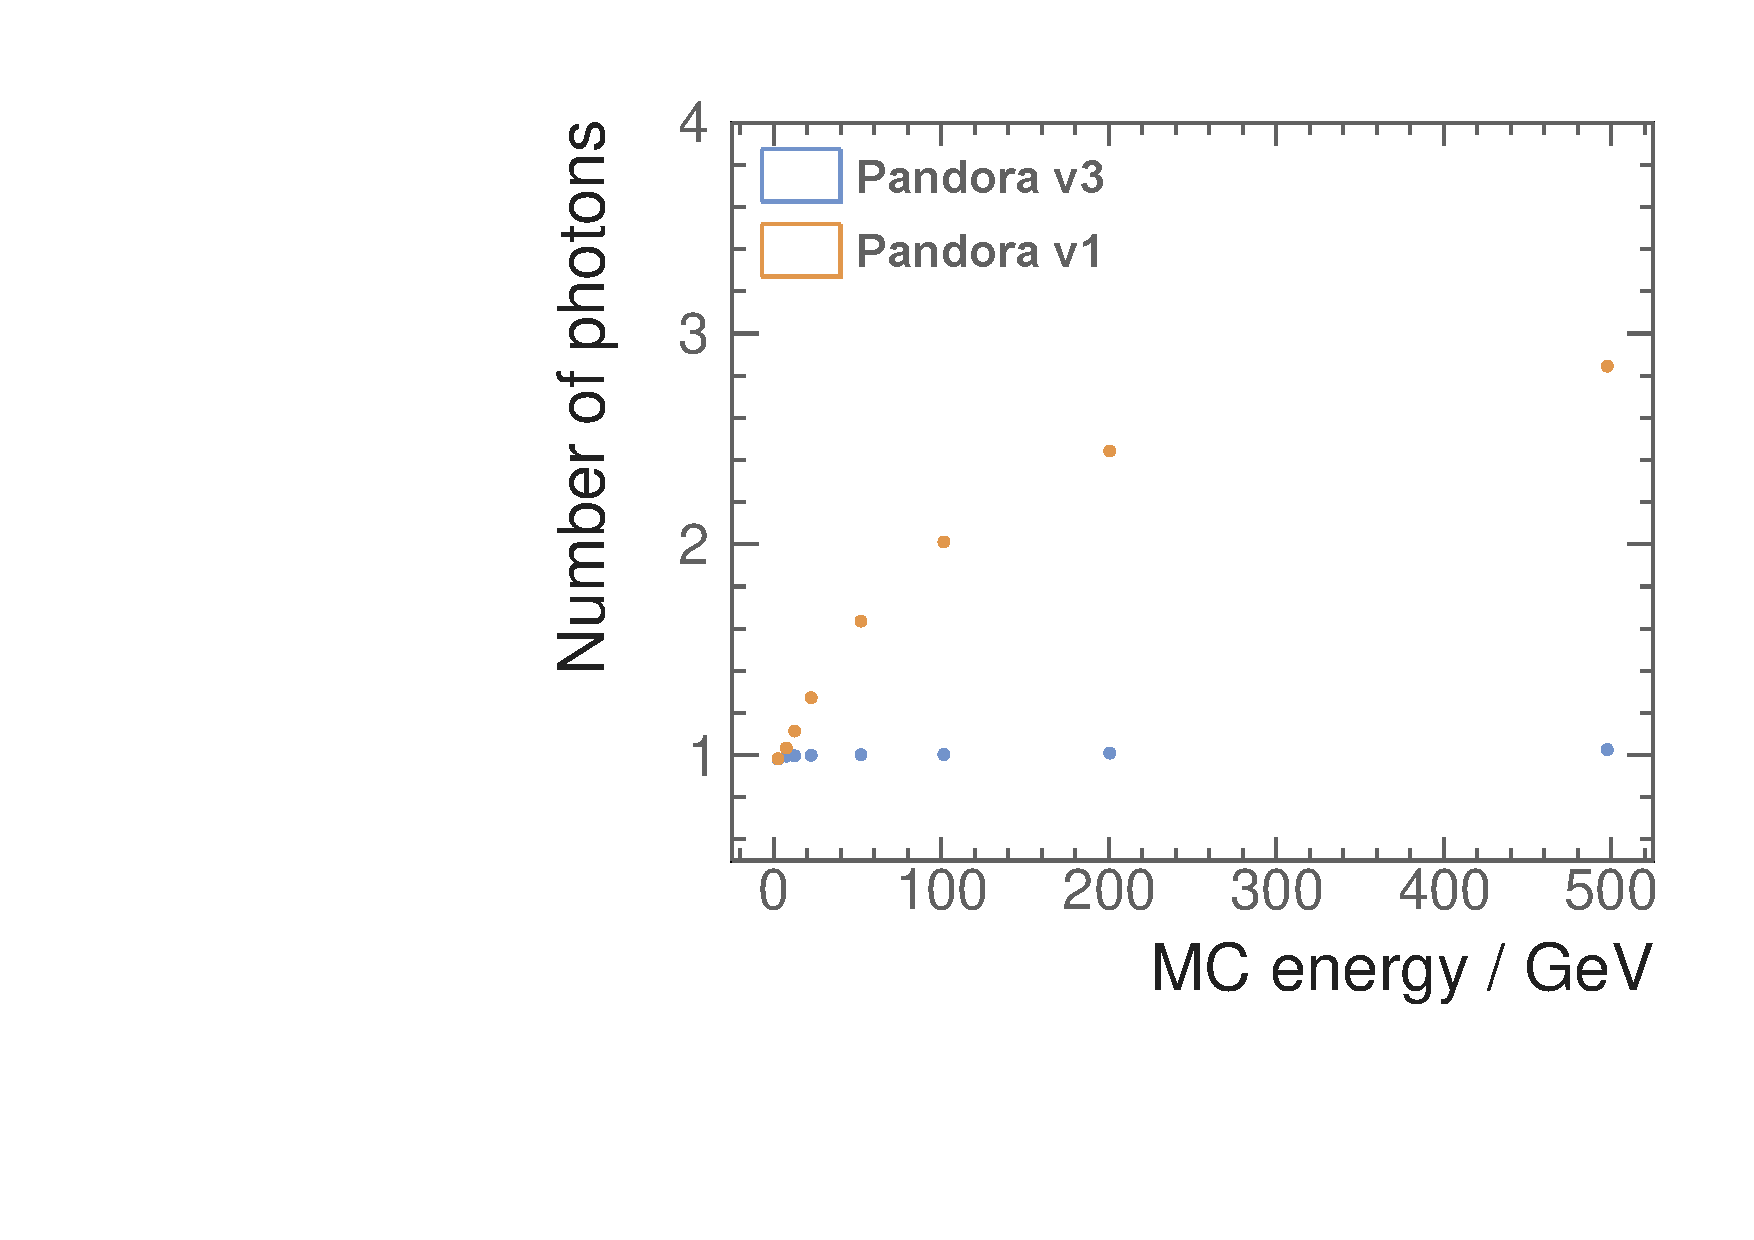
\includegraphics[width=\textwidth]{photon/SingleN_pedit.pdf}
        \caption{}
        \label{fig:photonSingleN_p}
    \end{subfigure}
    \begin{subfigure}[b]{0.45\textwidth}
        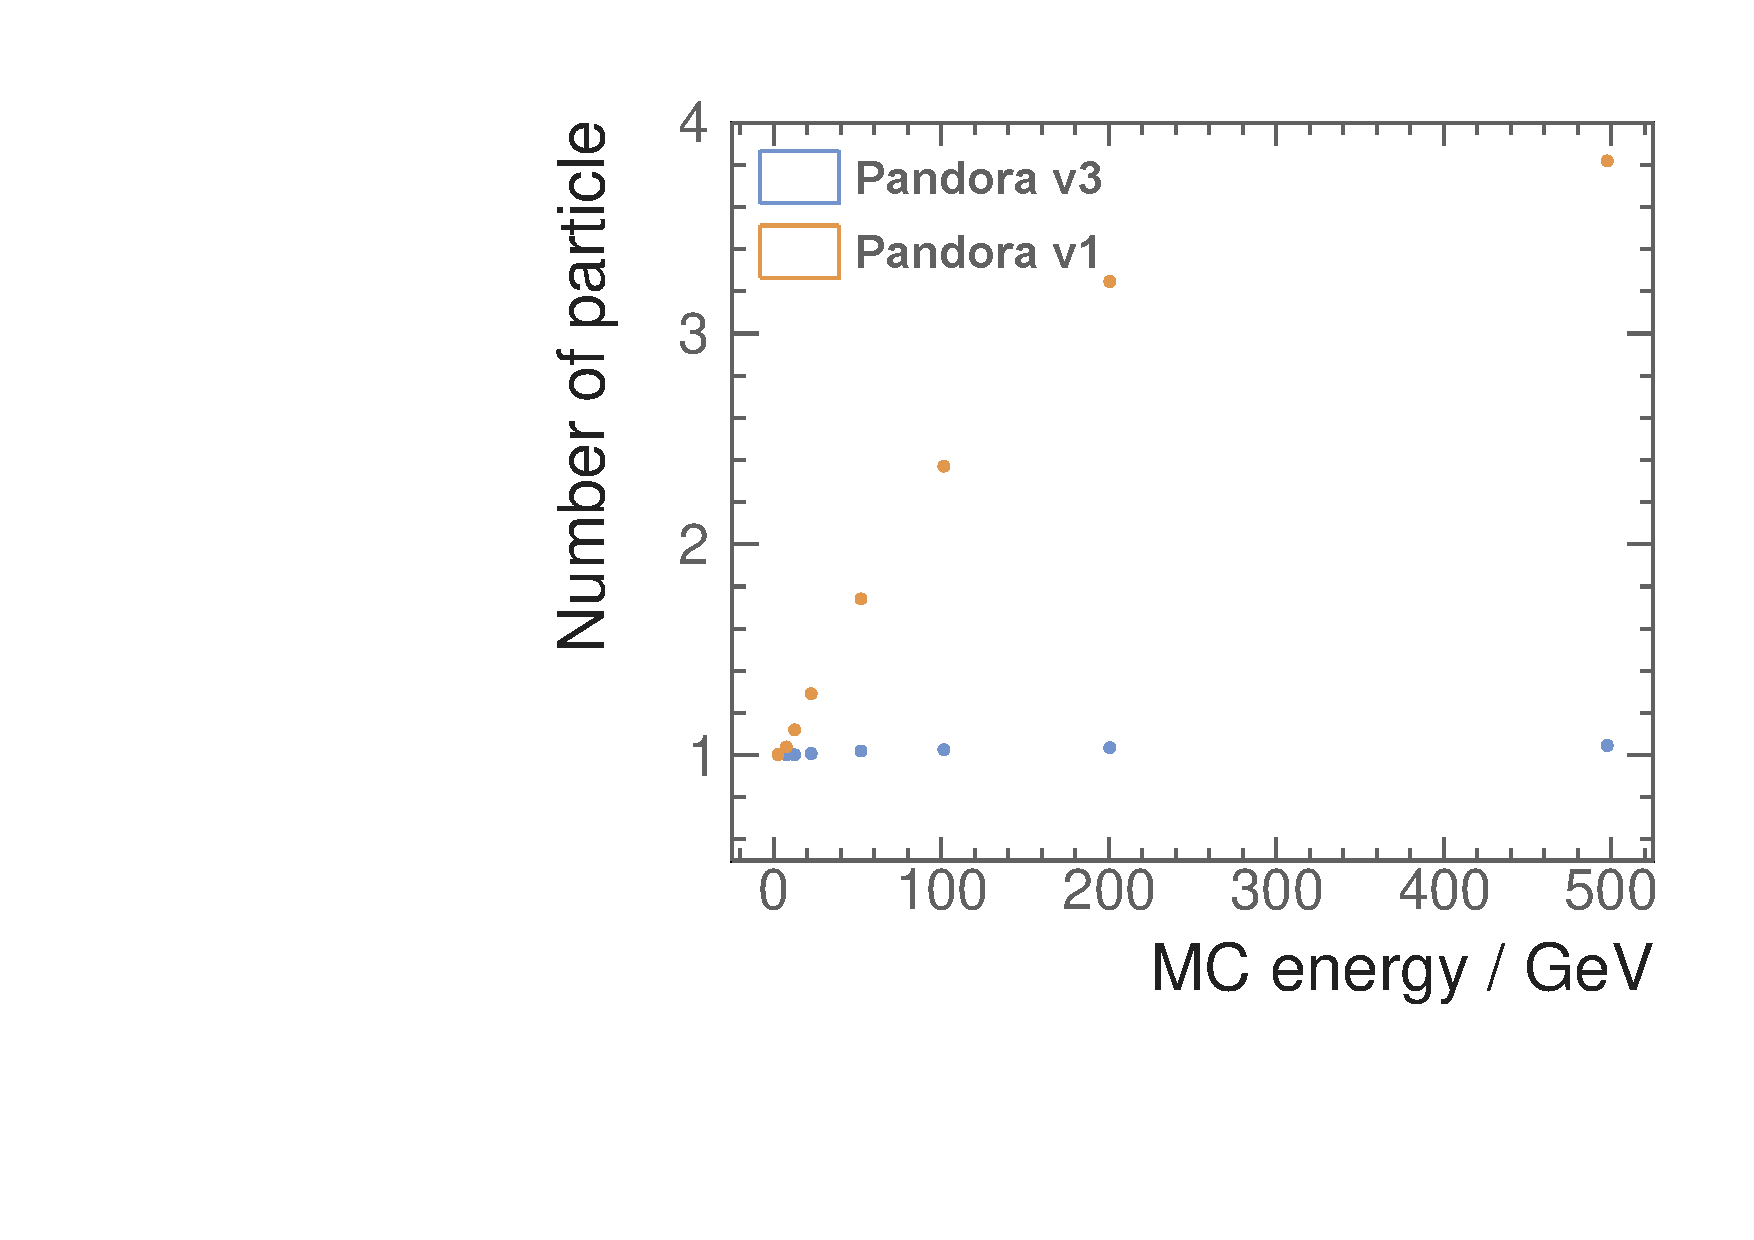
\includegraphics[width=\textwidth]{photon/SingleN_alledit.pdf}
        \caption{}
        \label{fig:photonSingleN_all}
    \end{subfigure}
\caption[Average number of reconstructed photons and reconstructed particles, as a function of their true energy using single photon sample.]
{\Figure{fig:photonSingleN_p} and \Figure{fig:photonSingleN_all} shows the average number of reconstructed photons and reconstructed particles, as a function of their true energy using a single photon per event sample. The top orange and bottom blue dots are reconstructed with \pandora version 1 and version 3. The photon reconstruction is changed in \pandora version 2.}
\label{fig:photonSingleN}
\end{figure}


\FIGURE{fig:photonSingleN_p} shows the reduction in fragments identified as photons, using a single photon per event sample. For the blue dots, the average number of photon stays below 1.05 even at high energy (true value 1). A similar trends shows in \Figure{fig:fig:photonSingleN_all}, where the extra fragments identified as neutral hadrons have taken into account. For a 100\,GeV photon, the average numbers of photon and particle are reduced to 1 from 2 and 2.4. For a 500\,GeV photon, the average numbers of photon and particle are reduced to 1.05 from 2.8 and 3.8.

\begin{figure}[tbph]
\centering
    \begin{subfigure}[b]{0.45\textwidth}
        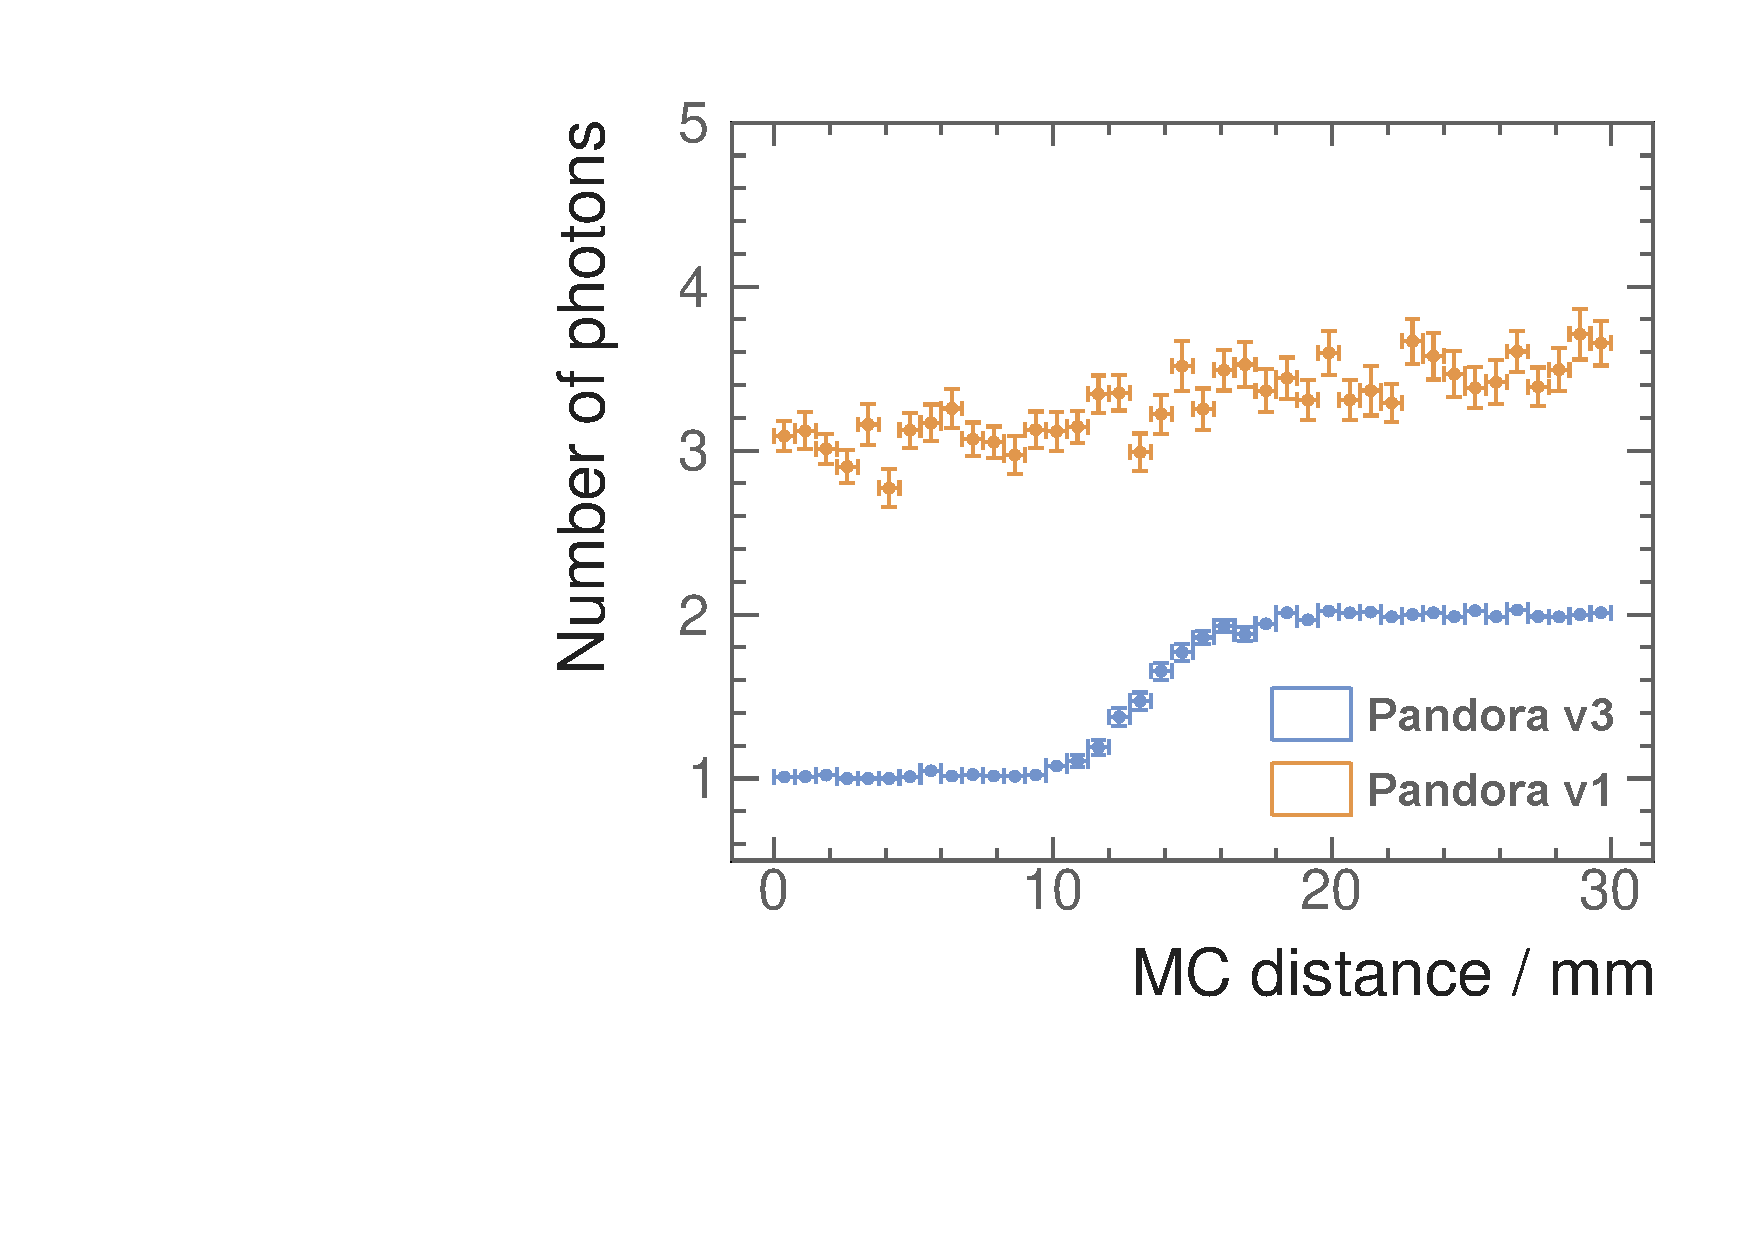
\includegraphics[width=\textwidth]{photon/DoubleCompareN_p3edit.pdf}
        \caption{}
        \label{fig:photonDoubleCompareN_p}
    \end{subfigure}
    \begin{subfigure}[b]{0.45\textwidth}
        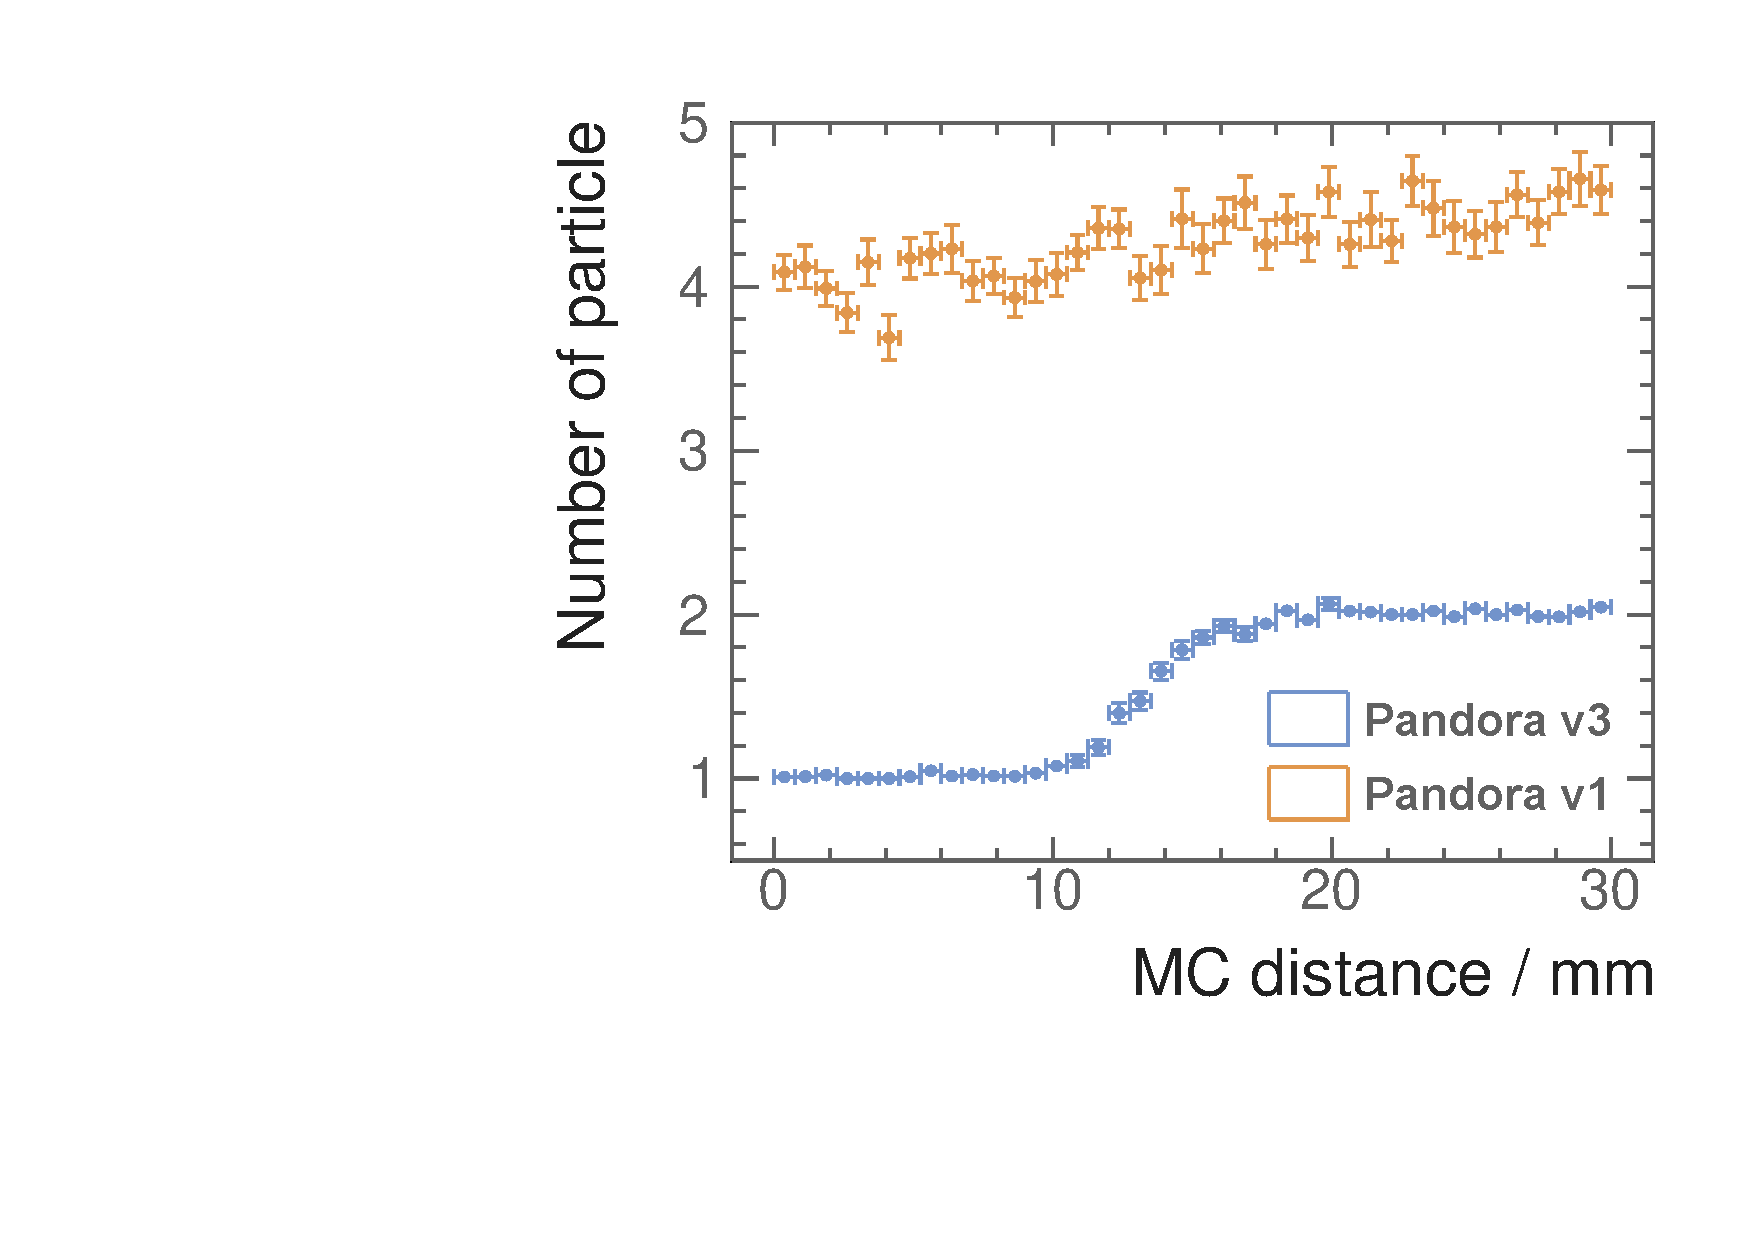
\includegraphics[width=\textwidth]{photon/DoubleCompareN_all2edit.pdf}
        \caption{}
        \label{fig:photonDoubleCompareN_all}
    \end{subfigure}
\caption[Average number of reconstructed photons and reconstructed particles, as a function of the MC distance separation.]
{\Figure{fig:photonDoubleCompareN_p} and \Figure{fig:photonDoubleCompareN_all} shows the average number of reconstructed photons and reconstructed particles, as a function of the MC distance separation in the calorimeter, using two photons of 500 and 50\,GeV per event sample. The top orange and bottom blue dots are reconstructed with \pandora version 1 and version 3. The photon reconstruction is changed in \pandora version 2.}
\label{fig:photonDoubleCompareN}
\end{figure}

\Figure{fig:photonDoubleCompareN} also illustrates a reduction in the photon fragments and the neutral hadron fragments using two photons of 500 and 50\,GeV per event sample. The figure shows the MC distance separation from 0 to 30\,mm, which corresponds to approximately 6 \ECAL square cell. This is a difficult test for fragment removal as high energy photons are more likely to create fragments and the imbalance in the two photon energies makes it more difficult to separate correctly.  In both \Figure{fig:photonDoubleCompareN_p} and \Figure{fig:photonDoubleCompareN_all}, the average numbers of photon and particle are below 2.05 at 30\,mm apart, which is significantly better than reconstruction in \pandora version 1. Two photons start to be resolved at 10\,mm apart, and fully resolved at 20\,mm apart. The resolution is better than reconstruction in \pandora version 1, which is difficult to extract due to excess fragments.




\begin{figure}[tbph]
\centering
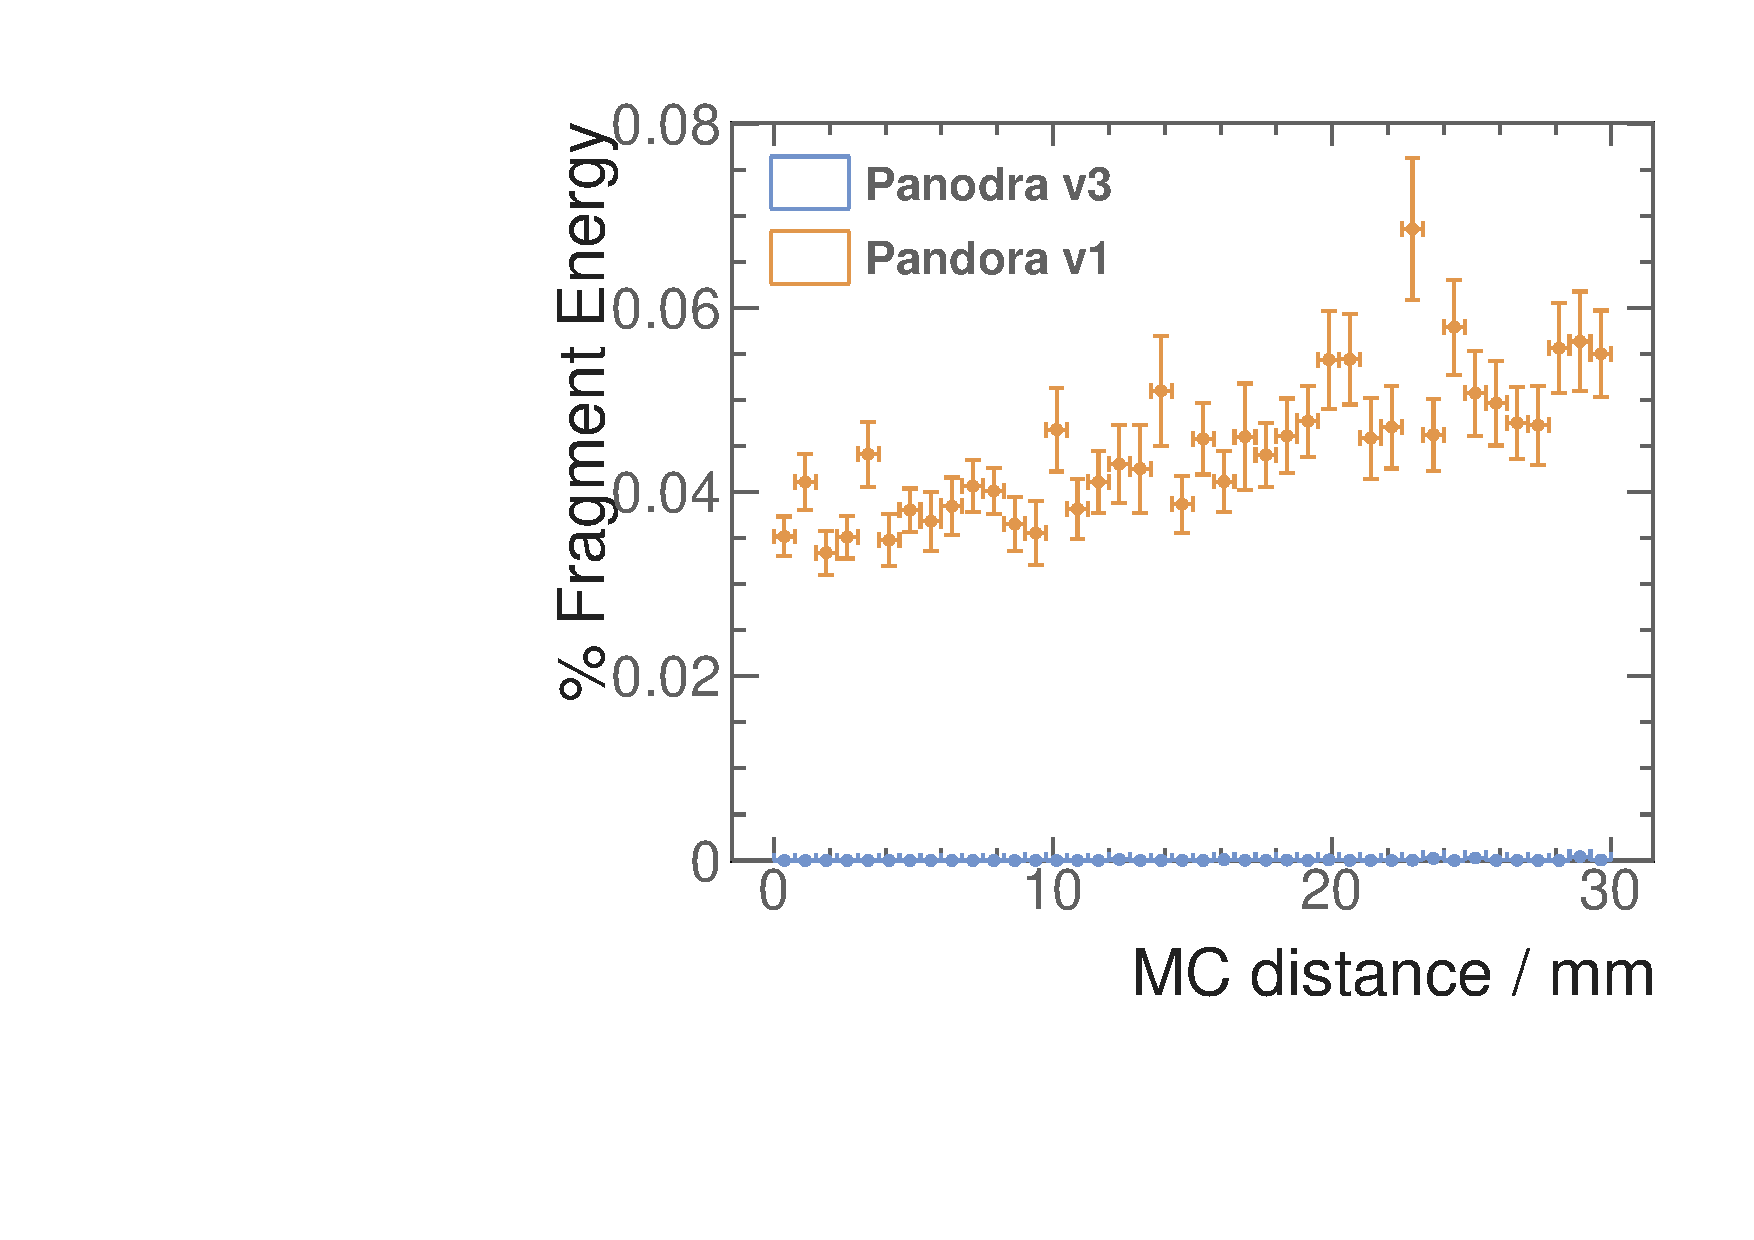
\includegraphics[width=0.45\textwidth]{photon/DoubleCompareFragEnergy.pdf}
\caption[Average fraction fragments energies of the total energy, as a function of the MC distance separation]
{\Figure{fig:photonDoubleFragEnergy} shows the average fraction fragments energies of the total energy, as a function of the MC distance separation in the calorimeter, using two photons of 500 and 50\,GeV per event sample. The top orange and bottom blue dots are reconstructed with \pandora version 1 and version 3. The photon reconstruction is changed in \pandora version 2.}
\label{fig:photonDoubleFragEnergy}
\end{figure}

Another metric to reflect the improvement in photon reconstruction is the fraction of the fragment energy to the total energy as function of the distance separation. Shown in \Figure{fig:photonDoubleFragEnergy}, using two photons of 500 and 50\,GeV per event sample, a reduction in fragment energy can be seen clearly. With improved reconstruction, the average fragment energy fraction is below 0.1\% up to 30\,mm apart, whilst around 5\% energy would be in fragments with reconstruction in \pandora version 1.




\begin{figure}[tbph]
\centering
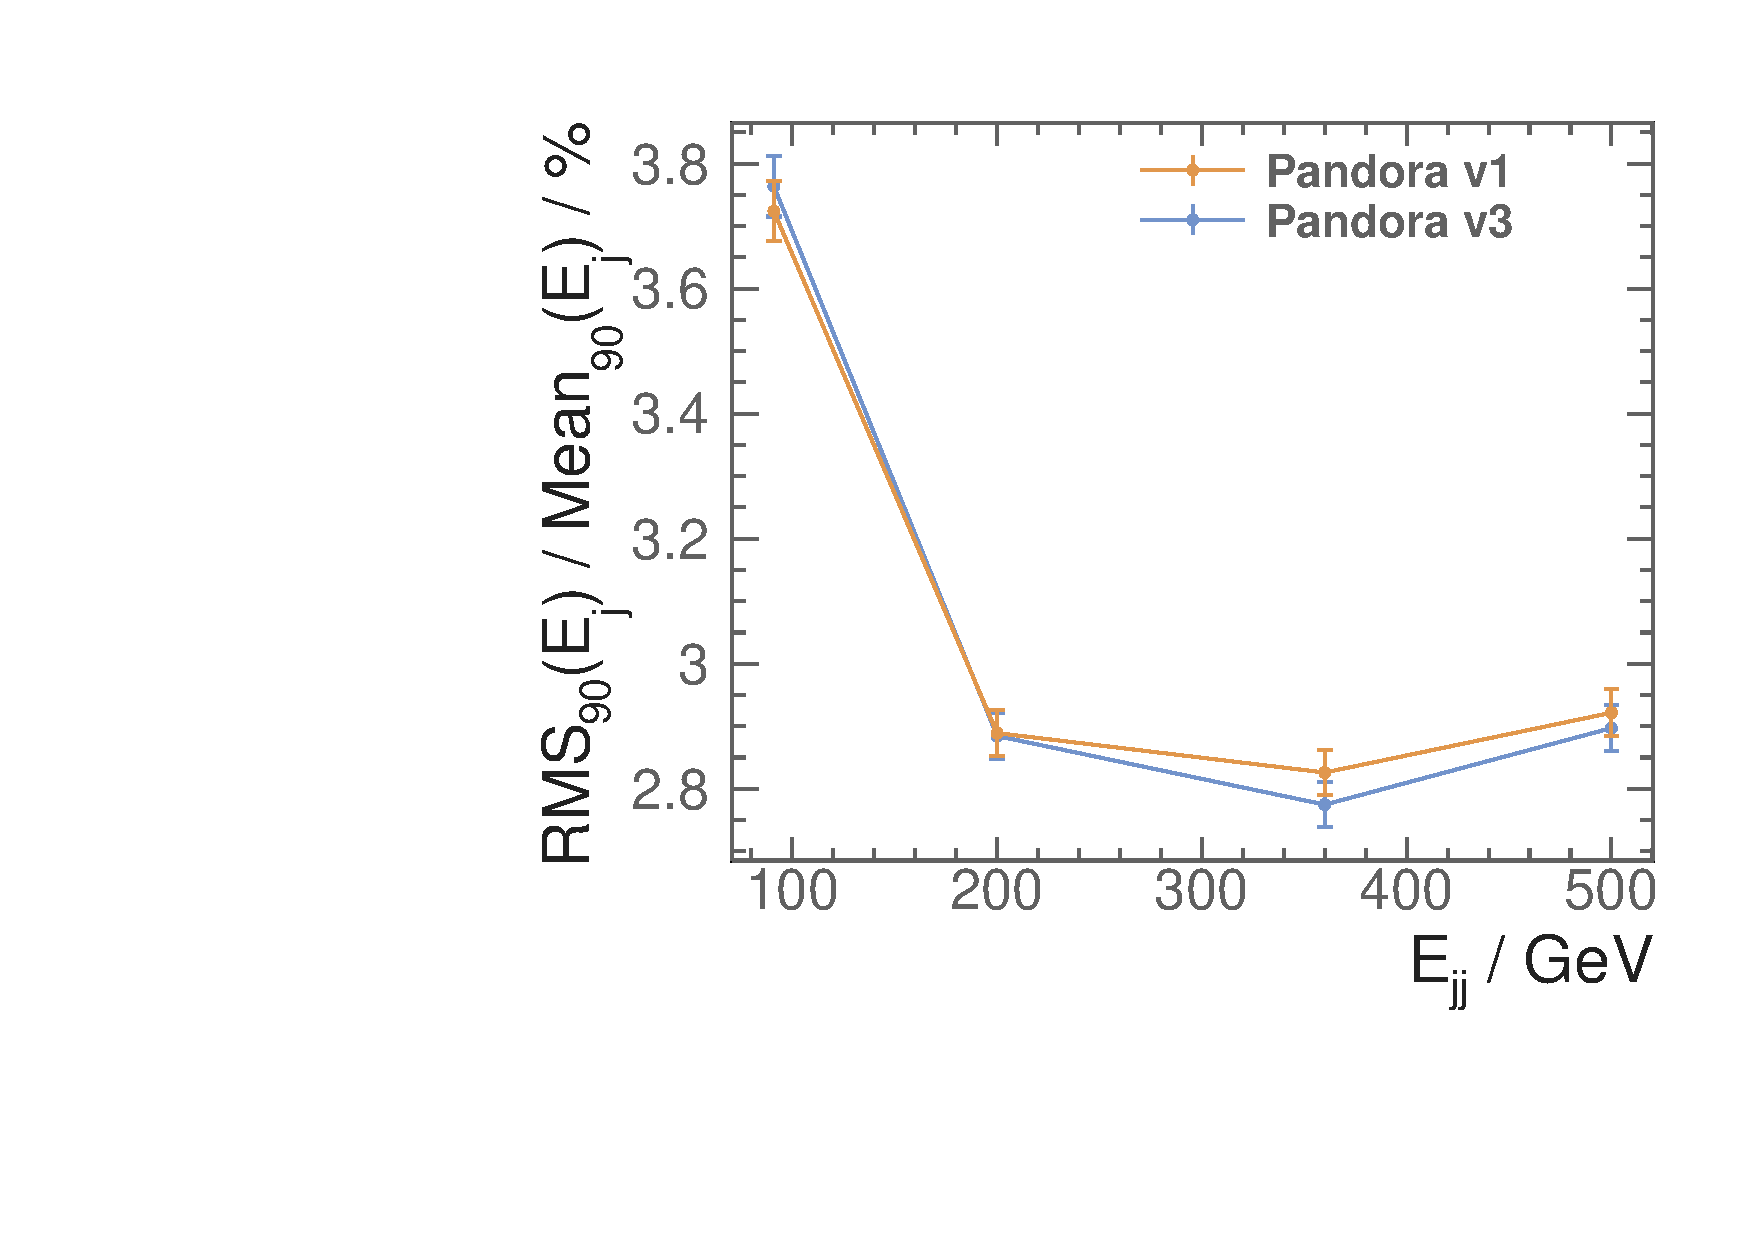
\includegraphics[width=0.45\textwidth]{photon/JERnew.pdf}
\caption[Jet energy resolution as a function of the di-jet energy]
{\Figure{fig:photonJER} shows jet energy resolution as a function of the di-jet energy using \Zuds sample at barrel region. The top orange and bottom blue dots are reconstructed with \pandora version 1 and version 3. The photon reconstruction is changed in \pandora version 2.}
\label{fig:photonJER}
\end{figure}

The improvement in completeness and resolution in photon reconstruction, as shown in single photon and double photon reconstruction, leads to a small improvement in the jet energy resolution at high energy. Jet energy resolution is defined as the root mean squared divided by the mean for the smallest width of distribution that contains 90\% of entries, using \Zuds sample at barrel region. The angular cut is to avoid the barrel/endcap overlap region. The light quark decay of the \PZ is used as \pandora does not attempt to recover missing momentum from semi-leptonic decay of heavy quarks. The di-jet energy is sampled at 91, 200, 360 and 500\,GeV. Shown in \Figure{fig:photonJER}, the jet energy resolutions are better at 360 and 500\,GeV with improved photon reconstruction. This is due to more aggressive photon reconstruction especially nearby tracks. 

The improvement of the photon is also demonstrated in \Chapter{chap:Tau}, where tau lepton decay modes are classified. Excellent photon reconstruction leads to a high classification rate.

\section{Breakdown of photon reconstruction improvement}



\begin{figure}[tbph]
\centering
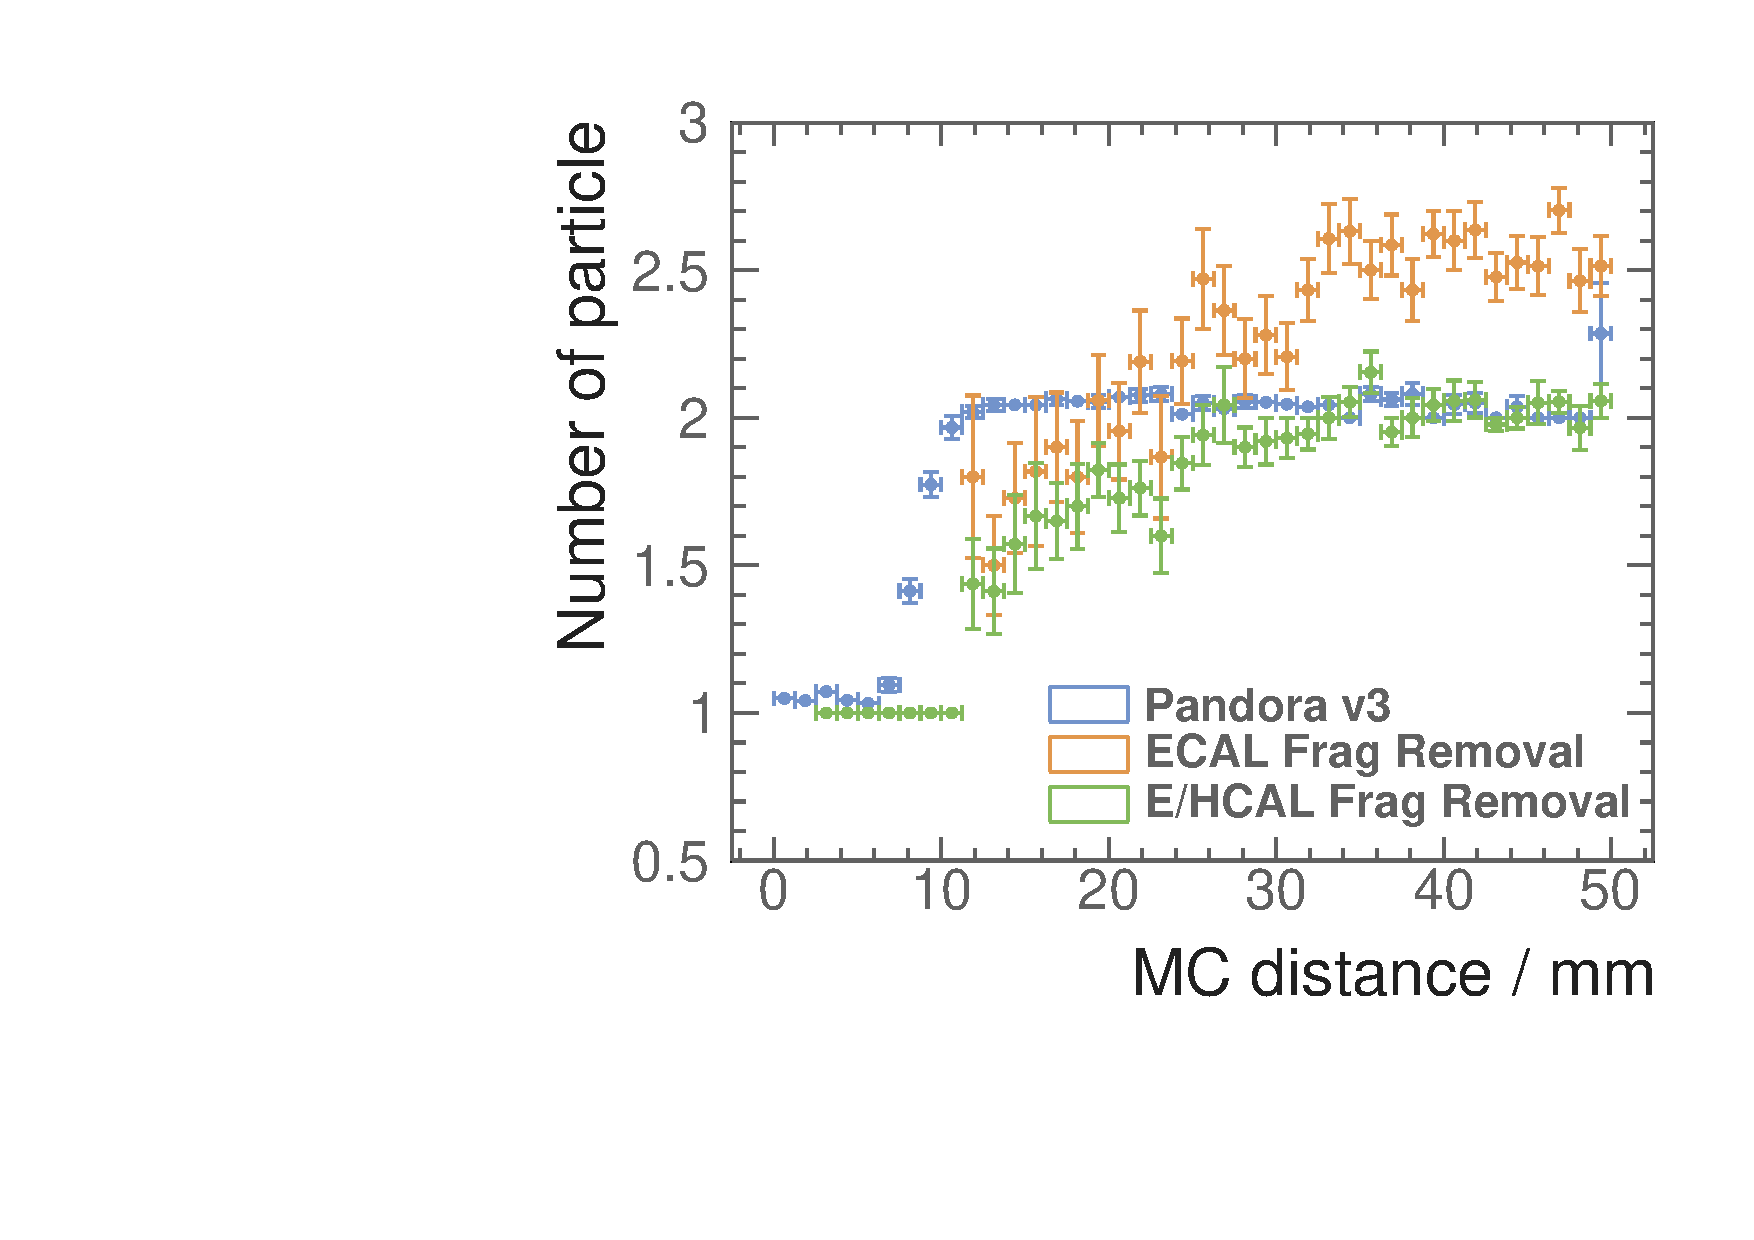
\includegraphics[width=0.45\textwidth]{photon/DoubleCompareAlgs.pdf}
\caption[Average number of photons, as a function of the MC distance separation for different algorithms combinations.]
{Figure shows the average number of photons, as a function of the MC distance separation in the calorimeter, using two photons of 500 and 500\,GeV per event sample. The blue, orange, and green dots are reconstructed with \pandora version 3, \pandora version 1 with fragment removal in the \ECAL (\Section{sec:photonFragRemoval}), and \pandora version 1 with fragment removal in the \ECAL and the \HCAL. The photon reconstruction is changed in \pandora version 2.}
\label{fig:photonDoubleCompareAlgs}
\end{figure}

As stated before, photon reconstruction algorithm in \Section{sec:photonRecostrcution} and photon splitting algorithm in \Section{sec:photonSplitting}  improves the photon completeness and the photon pair resolution. The fragment removal algorithm in \Section{sec:photonFragRemoval} removes fragments in the \ECAL. High energy fragment removal algorithm in \Section{sec:photonHighEFragRemoval} removes fragments in the \HCAL. To show the incremental improvement, the average number of particle for a high energy photon pair, 500 - 500\,GeV is shown in \Figure{fig:photonDoubleCompareAlgs}. 

With fragment removal algorithm in the \ECAL, the number of fragment is reduced significantly (comparing with \Figure{fig:photonDoubleCompareN_all}). With the energy fragment removal in the \HCAL, the number of fragments are reduced further. With all algorithms implemented, the reduction in fragments is most significant. At 40\,mm apart, with both fragment removal algorithms (green dots), there is less than 0.05 fragment per photon pair. 

The introduction of the revised photon reconstruction and photon splitting improves the photon separation resolution. Photons pair starts to be resolved at 5\,mm for 500 - 500\,GeV pair and fully resolved at 15\,mm.

\section{Photon reconstruction performance}

In \Section{sec:photonPerformanceCompare}, the improved performance of the photon reconstruction is demonstrated with different metrics, using single photon, double photons and jet samples. In this section, the features of the photon reconstruction will be described.

For simple samples such as two photons per event, there are very few fragments. Shown in \Figure{fig:photonDoubleCompareN_pN_all} for 500 and 50\,GeV photons pair sample, the average number of photons and particles beyond 20\,mm apart is less than 2.05. 

\begin{figure}[tbph]
\centering
    \begin{subfigure}[b]{0.45\textwidth}
        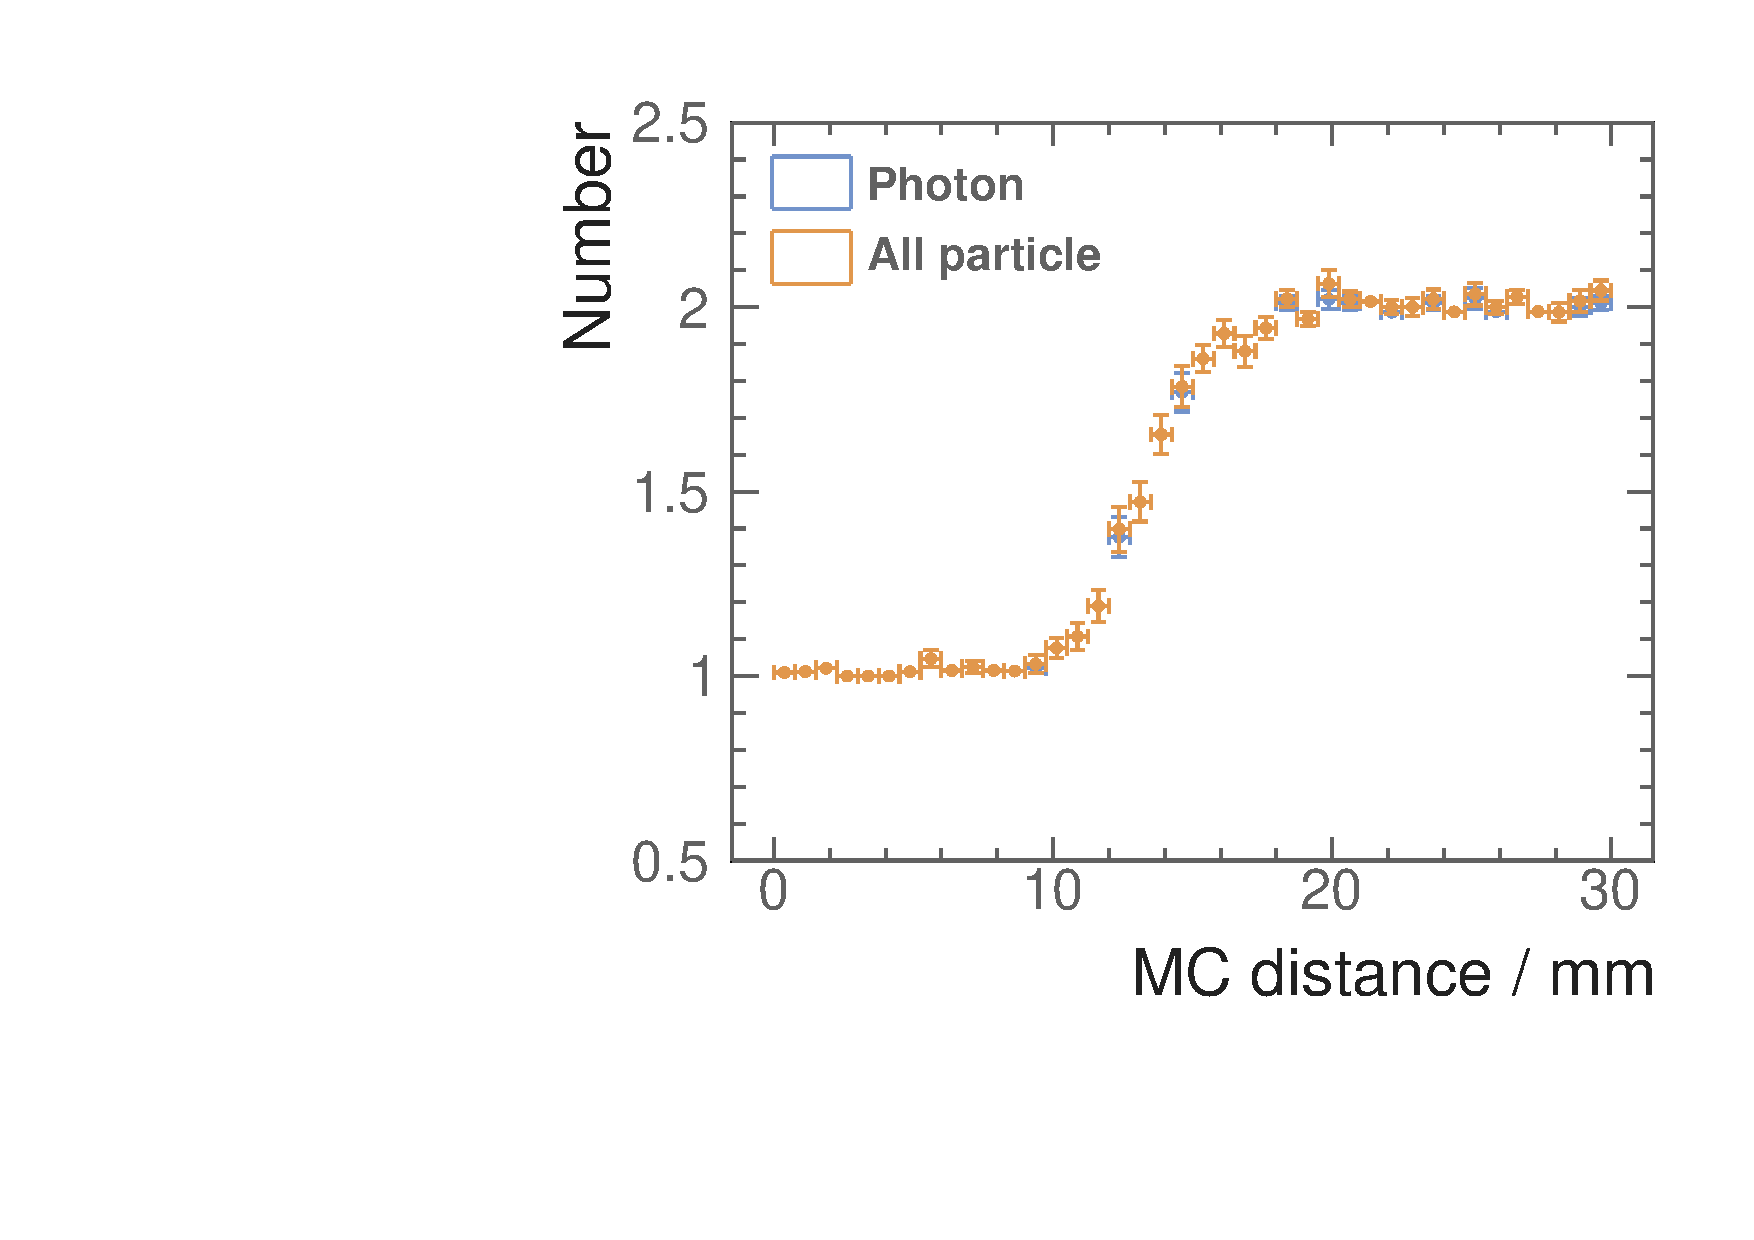
\includegraphics[width=\textwidth]{photon/DoubleN_pN_all.pdf}
        \caption{}
        \label{fig:photonDoubleCompareN_pN_all}
    \end{subfigure}
    \begin{subfigure}[b]{0.45\textwidth}
        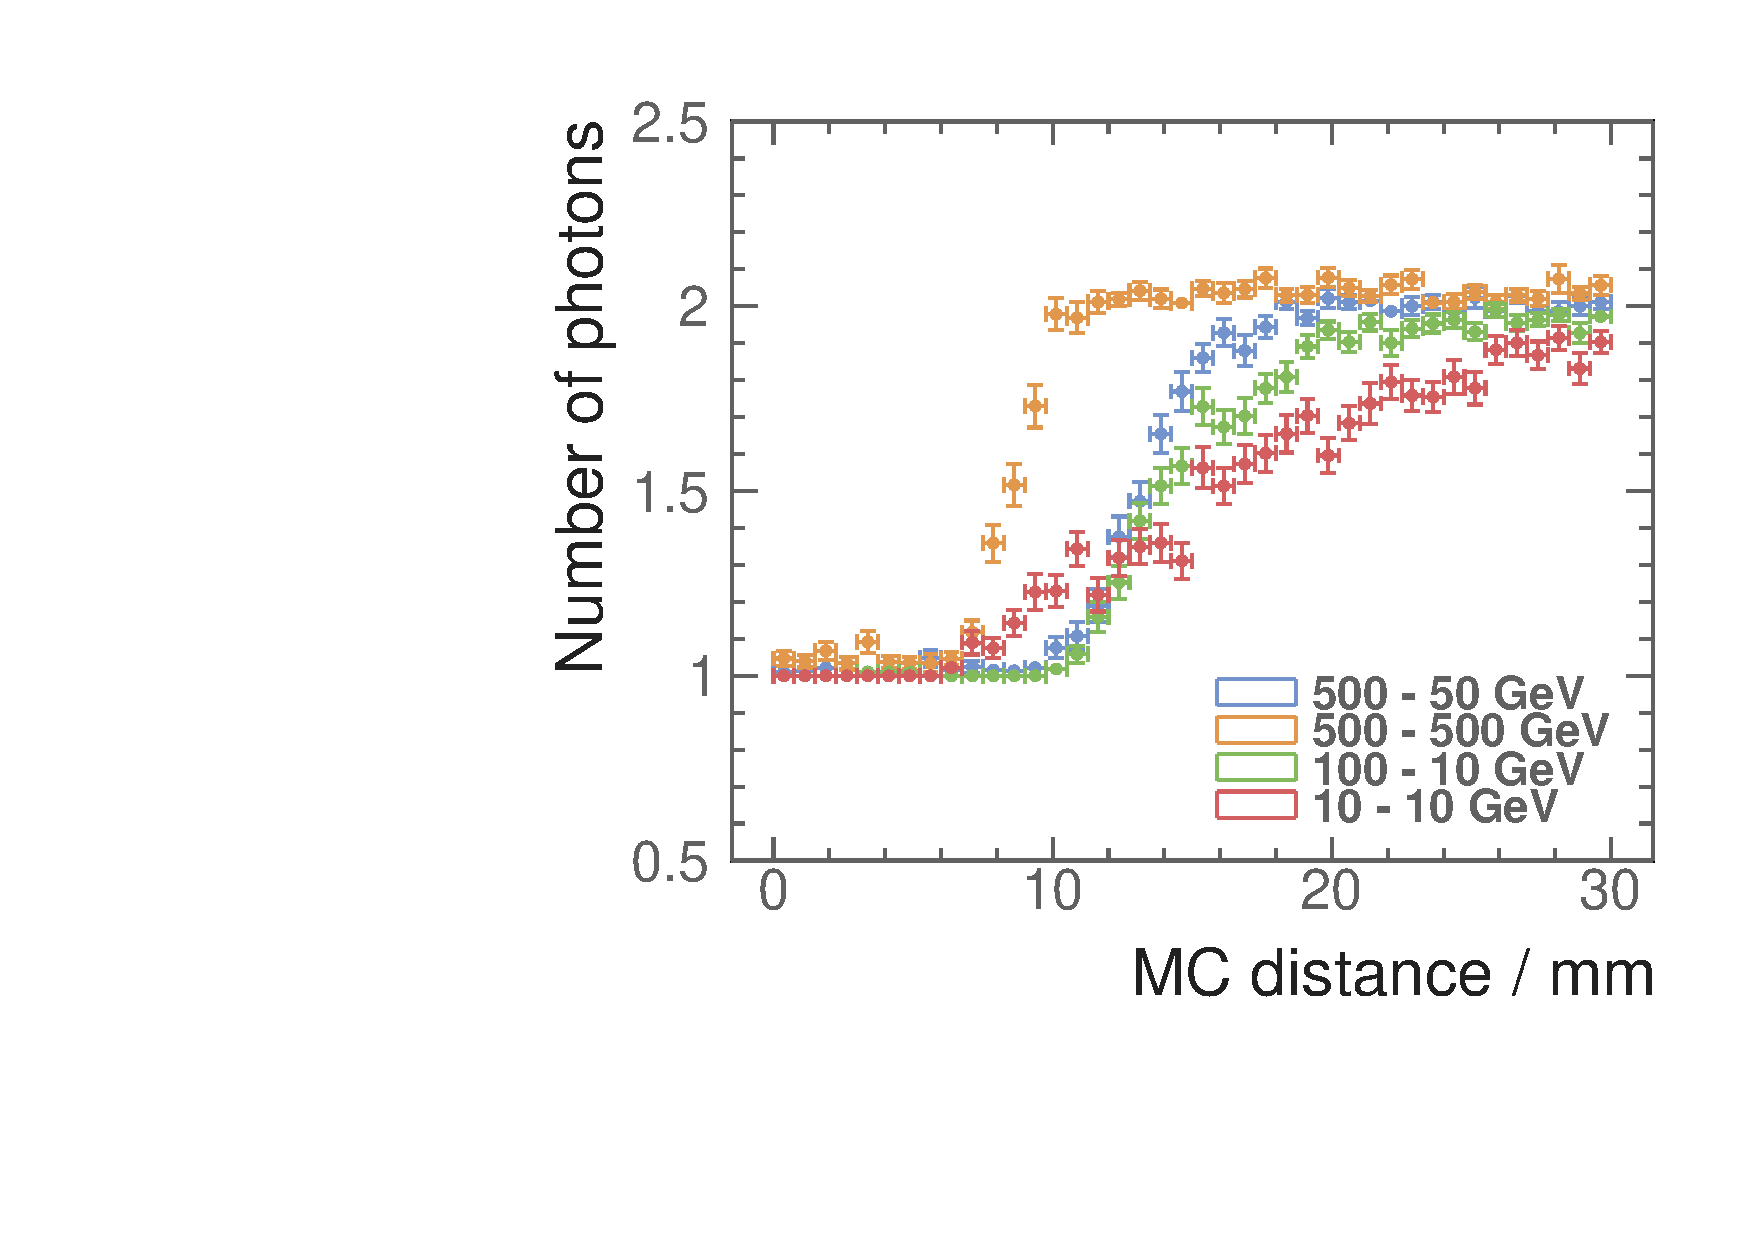
\includegraphics[width=\textwidth]{photon/DoubleCompareEnergies.pdf}
        \caption{}
        \label{fig:photonDoubleCompareEnergies}
    \end{subfigure}
\caption[Average numbers of photon and particle using two photons of 500 and 50\,GeV per event sample and with different energy pairs.]
{\Figure{fig:photonDoubleCompareN_pN_all} shows the average numbers of photon and particle using two photons of 500 and 50\,GeV per event sample. \Figure{fig:photonDoubleCompareEnergies} shows the  average numbers of photon for four different photon pairs: 500 - 50, 500 - 500, 100 - 10 and 10 - 10\,GeV.}
\label{fig:photonDoublePerformance}
\end{figure}

The resolving power of a photon pair depends on energies of two photons. \Figure{fig:photonDoubleCompareEnergies} is an example of average number of photon reconstructed for differen photon pairs. When the energies of two photons are similar, the resolving distance is shorter. This is because that the two photon showers have similar sizes, and the peak finding algorithm can exploit the symmetry. For example, 500 - 500\,GeV photon pair and 10 - 10\,GeV photon pair start to be resolved at 6\,mm apart, which is about 1 \ECAL cell. The asymmetrical photon pair,  500 - 50\,GeV and  100 - 10\,GeV pair, starts to be resolved at 10\,mm apart, which is about 2 \ECAL cell.

For the energetic photon, it is more difficult to remove fragments, but it is easier to identify the photon. The electromagnetic shower core is more dominant than the peripherals. Therefore separating two energetic photons is easier than separating two low energy photons. This can be seen in \Figure{fig:photonDoubleCompareEnergies}. At 20\,mm apart, two photons in  500 - 500\,GeV pair are fully resolved, where approximately 60\% of two photons in 10 - 10\,GeV pair are resolved.

